%!TEX root=./LIVRO.tex
\chapter{1. A interpretação de textos}

\coment{Neste módulo, os alunos deverão ser guiados durante o processo de
leitura. É importante mostrar à turma os passos necessários para a total
compreensão de um texto, começando pelo tema. Posteriormente, você deve salientar como informações tanto explícitas quanto
implícitas podem ser encontradas em um mesmo texto.\\
Habilidades da BNCC: EF35LP03, EF15LP03, EF35LP04, EF35LP05 e EF05LP08.}

\colorsec{Habilidades do SAEB}

\begin{itemize}
\item Identificar a ideia central do texto.

\item Localizar uma informação explícita.

\item Inferir informações implícitas em textos.

\item Inferir o sentido de palavras ou expressões em textos.

\item Reconhecer em textos o significado de palavras derivadas a partir de
seus afixos.
\end{itemize}

\begin{figure}[htpb!]
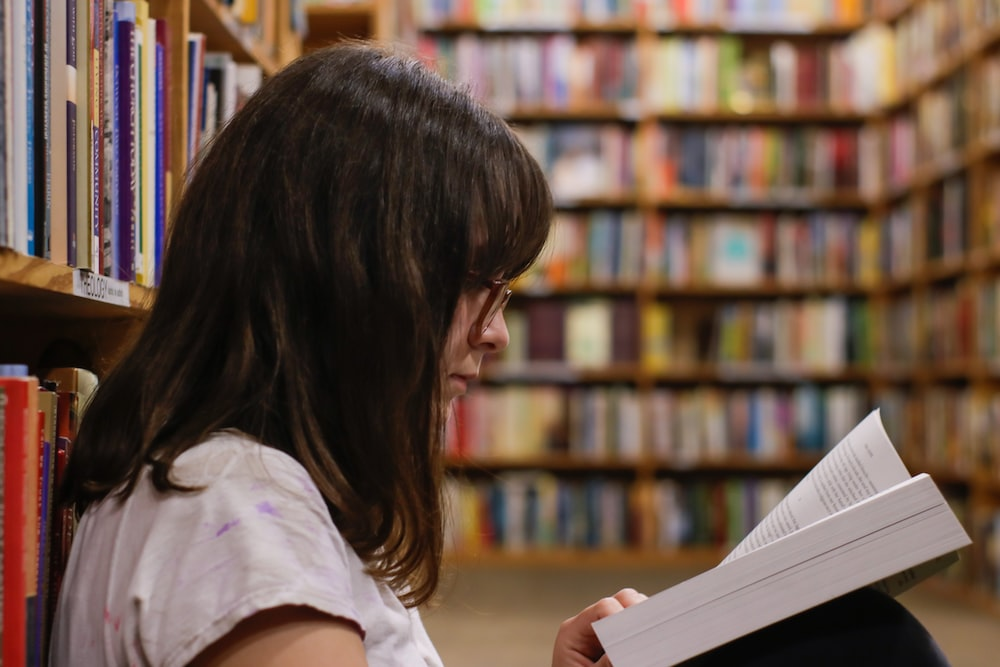
\includegraphics[width=.5\textwidth]{./imgs/img1.jpg}
\caption{Fonte: https://unsplash.com/pt-br/fotografias/kcT-7cirBEw. Acesso 20/02/2023.}
\end{figure}

\conteudo{Existem diversas maneiras de nos comunicarmos. Uma delas se dá pela
criação de textos que podem ser veiculados em diferentes meios, como
sites de internet, jornais, revistas, livros, cartazes e muito mais. Para nos mantermos
informados, é importante desenvolvermos o hábito da leitura e
consultarmos muitas fontes a fim de termos acesso a pontos de vista
distintos!

Ao entrarmos em contato com um texto, primeiro devemos identificar seu tema e seu assunto. Leia o texto a seguir.

\begin{quote}
\textbf{A cultura brasileira}

A cultura brasileira é muito diversa, uma mistura de influências
indígenas, africanas e europeias. Essa diversidade pode ser percebida em
áreas como a música, a dança e a religião. O Brasil é conhecido
mundialmente por seus estilos musicais, como o samba, o forró e a
bossa nova, e pela dança, com destaque para o carnaval e o frevo.
Além disso, a culinária brasileira é repleta de sabores e aromas únicos,
com pratos como a feijoada, o churrasco e a moqueca.
\fonte{Texto escrito para este material.}
\end{quote}

Consegue identificar o tema do texto? Trata-se de um breve panorama
sobre a cultura brasileira, como podemos constatar logo na primeira
linha. Também é possível encontrarmos informações específicas, como a
riqueza dos estilos musicais encontrados em nosso país.

É importante destacarmos também a presença de informações implícitas em
um texto, ou seja, informações que podem ser obtidas por meio da leitura
ainda que não sejam citadas explicitamente. Nesse texto, embora isto
não seja afirmado, é possível chegarmos à conclusão de que a cultura é
um aspecto muito importante de uma nação, pois permite que associemos
características específicas a um povo.

Um texto também proporciona ao leitor o aprendizado da língua. A partir
desse trecho, conhecemos palavras como ``frevo'' e
``moqueca'', que nomeiam importantes aspectos da cultura brasileira.

Por fim, um texto também permite que o leitor aprenda mais sobre a
estrutura das palavras. O termo ``brasileira'', por exemplo, indica algo ou alguém proveniente do Brasil. Dessa forma, chegamos
à conclusão de que uma terminação como ``-eiro'' (que, no texto, aparece na forma feminina ``-eira'') pode ser utilizada
quando necessitamos construir uma relação de pertencimento.}

\colorsec{Atividades}

\num{1}  Ao lermos um texto pela primeira vez, qual aspecto devemos identificar imediatamente?

\coment{Devemos identificar o tema trabalhado no texto.}

\linhas{2}

\num{2} Leia o trecho a seguir e identifique o tema discutido.

\begin{figure}[htpb!]
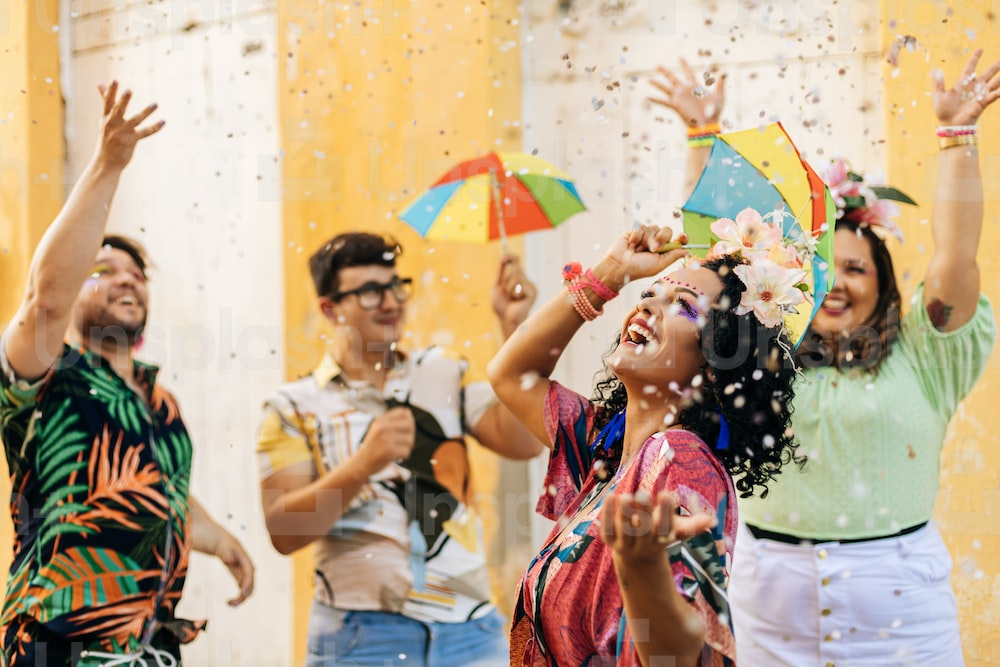
\includegraphics[width=.5\textwidth]{./imgs/img2.jpg}
\caption{Fonte: https://unsplash.com/pt-br/fotografias/soH7UcycvKA. Acesso em: 20/02/2023.}
\end{figure}

\begin{quote}
O Carnaval brasileiro é uma das festas mais animadas e coloridas do
mundo. Celebrado anualmente, geralmente em fevereiro ou março, é um
momento de grande festa.
\fonte{Texto escrito para este material.}
\end{quote}

\linhas{2}

\coment{O texto trata da comemoração do Carnaval no Brasil.}

\num{3} De acordo com o texto, quando o Carnaval é comemorado no Brasil?

\linhas{1}

\coment{O Carnaval é comemorado geralmente em fevereiro ou março.}

\num{4} Assinale V para o que for verdadeiro e F para o que for falso.

\begin{boxlist}
\item Não podemos obter informações específicas em um texto. \coment{F}

\item Podemos aprender novas palavras por meio da leitura de um texto. \coment{V}

\item Não é importante conhecermos o tema de um texto. \coment{F}

\item É possível deduzirmos ou inferirmos informações a partir de um texto. \coment{V}
\end{boxlist}

Leia o texto a seguir e responda às questões de 5 a 7.

\begin{quote}
Machado de Assis foi um dos maiores escritores da literatura
brasileira. Ele nasceu no Rio de Janeiro, em 1839, e viveu em uma época
de grandes transformações no país, como a transição da monarquia para a
república e o fim da escravidão.
\fonte{Texto escrito para este material.}
\end{quote}

\num{5} Encontre no texto o ano e a cidade de nascimento do escritor Machado de Assis.

\linhas{2}
\coment{Machado de Assis nasceu em 1839 no Rio de Janeiro.}

\num{6} De acordo com o texto, quais transformações importantes ocorreram na época de Machado de Assis?

\linhas{3}
\coment{Machado de Assis foi contemporâneo à transição da monarquia para a
república e ao fim da escravidão.}

\num{7} Em ``escritores'', encontramos a terminação ``-tor'', que forma muitas palavras em língua portuguesa. Usando essa terminação, forme novas palavras relacionadas a estas:

\begin{escolha}
\item Agricultura: \preencher \coment{agricultor.}

\item Pintura: \preencher \coment{pintor.}

\item Canto: \preencher \coment{cantor.}

\item Construção: \preencher \coment{construtor.}
\end{escolha}

\num{8} Leia o texto a seguir e assinale V para o que for verdadeiro e F para o que for falso.

\begin{quote}
Luciana andava tranquilamente pela rua quando se lembrou de algo muito
importante: precisava comprar ração de gato! Estacionou, então, na
garagem de uma loja de animais e procurou a marca favorita de comida de
Lili.
\fonte{Texto escrito para este material.}
\end{quote}

\begin{boxlist}
\item É possível concluir que Luciana deve ter uma gata. \coment{V}

\item Luciana andava a pé pela rua quando parou para comprar ração de gato. \coment{F}

\item Lili é o nome da gata que aparece mencionada no texto. \coment{V}
\end{boxlist}

\coment{O aluno deve ser capaz de identificar informações implícitas no texto.}

Leia o texto a seguir e responda às questões 9 e 10.

\begin{quote}
A bossa nova é um dos movimentos musicais mais importantes do Brasil e
um dos mais reconhecidos internacionalmente. Ela surgiu na década de
1950, no Rio de Janeiro, e foi influenciada por outras formas de arte,
incluindo o jazz, o samba e a poesia.
\fonte{Texto escrito para este material.}
\end{quote}

\num{9} Encontre, no texto, fatores que influenciaram o surgimento da bossa nova.

\linhas{3}
\coment{A bossa nova foi influenciada por formas de arte como o jazz, o samba e a poesia.}


\num{10} Como a terminação ``-mente'', em ``internacionalmente'', pode ser explicada com relação ao sentido que ela acrescenta à palavra primitiva?

\linhas{5}
\coment{A terminação ``-mente'' é um sufixo de formação de advérbios, como os de modo, que é o caso de ``internacionalmente''. Pode-se explicar a palavra derivada com a expressão ``de modo internacional''.}


\colorsec{Treino}

\num{1} Leia o texto.

\begin{figure}[htpb!]
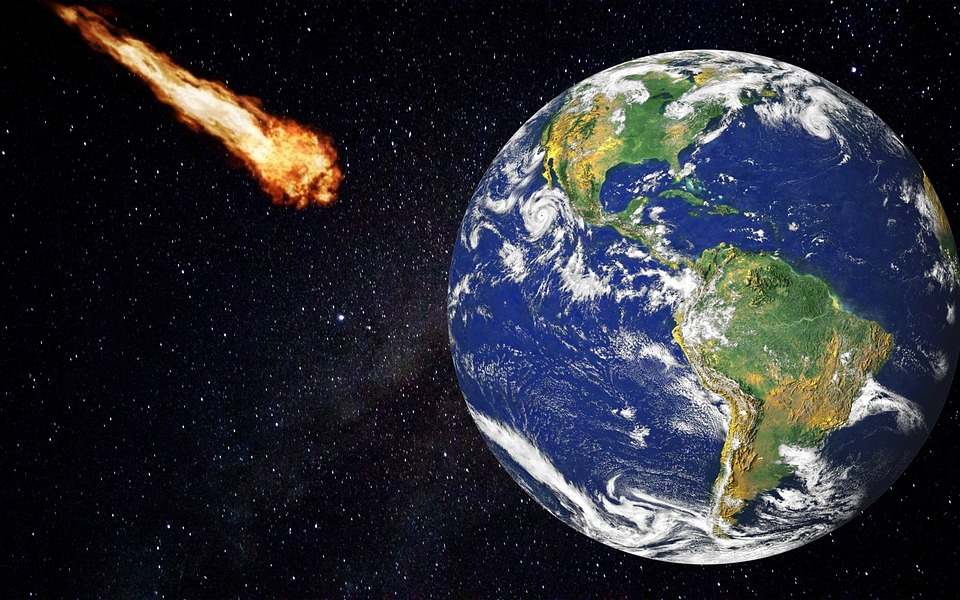
\includegraphics[width=.5\textwidth]{./imgs/img3.jpg}
\caption{Fonte: https://pixabay.com/pt/photos/aster\%c3\%b3ide-cometa-meteorito-3628185/. Acesso em 20/02/2023.}
\end{figure}

\begin{quote}
\textbf{Asteroide de mais de 1 km vai passar ``próximo'' da Terra nesta
quarta: entenda classificação da Nasa}

Um asteroide com cerca de \textbf{1,2 km} de diâmetro vai passar
``relativamente perto'' da Terra {[}...{]}. Mas
isso não é motivo para alarde.

O chamado 199145 (2005 YY128) não representa nenhuma ameaça para nós
porque, segundo a Nasa, o
objeto passará a cerca de 12 vezes a distância média entre a Terra e a
Lua, a 4,5 milhões de quilômetros.

{[}...{]}.

\fonte{Roberto Peixoto. Asteroide de mais de 1 km vai passar ``próximo'' da Terra nesta quarta: entenda classificação da Nasa. G1. Disponível em: \emph{https://g1.globo.com/ciencia/noticia/2023/02/15/asteroide-de-mais-de-1-km-vai-passar-proximo-da-terra-nesta-quarta-15-entenda-classificacao-da-nasa.ghtml}. Acesso em: 20 fev. 2023.}
\end{quote}

Assinale o que se pode afirmar de acordo com o texto.

\begin{escolha}
\item A passagem do asteroide será perigosa para a Lua.

\item Os habitantes do planeta Terra devem ficar muito preocupados com a
aproximação do asteroide.

\item A aproximação do asteroide não representa perigo para o planeta
Terra.

\item O asteroide possui uma extensão inferior a 1 km.
\end{escolha}

\coment{SAEB: Localizar informação explícita.
BNCC: EF15LP03 - Localizar informações explícitas em textos.

a) Incorreta. O texto apenas menciona a Lua para comparar a distância
entre nosso planeta e esse satélite e a rota do asteroide.
b) Incorreta. O texto afirma que não há motivo para alarde na Terra.
c) Correta. De acordo com o texto, o asteroide não representa nenhuma
ameaça para os habitantes do planeta Terra.
d) Incorreta. Segundo o texto, o asteroide apresenta cerca de 1,2 km de
extensão.}

\num{2} Leia o texto.

\begin{quote}
\textbf{Múmia extraordinariamente conservada}

Escavando túmulos na antiga necrópole de Saqqara, no Egito, arqueólogos descobriram a múmia de um homem chamado Hekashepes. Ele deve ter vivido por volta do ano 2300 a.C.

O que espantou positivamente os estudiososo é que, pensando no período da mumificação, os restos mumificados foram encontrados extraordinariamente bem conversados, dentro de um sarcófago de calcário.

\fonte{Fonte de pesquisa: Maiken Mosleth King. Arqueólogos descobrem múmia de mais de 4 mil anos coberta em ouro. BBC. Disponível em: \emph{https://www.bbc.com/portuguese/articles/cq5gge11dldo}. Acesso em: 20 fev. 2023.}
\end{quote}

O fato de a múmia estar extraordinariamente bem preservada para o período
indica que os arqueólogos

\begin{escolha}
\item não costumam encontrar múmias bem preservadas.

\item sempre encontram múmias bem preservadas.

\item pela primeira vez encontraram uma múmia.

\item não consideram a descoberta relevante.
\end{escolha}

\coment{SAEB: Inferir informações implícitas em textos.
BNCC: EF35LP04 - Inferir informações implícitas nos textos lidos.

a) Correta. O fato de o texto salientar a preservação da múmia implica
que, normalmente, os achados não apresentam as mesmas características.
b) Incorreta. As informações encontradas no texto implicam exatamente o
contrário.
c) Incorreta. O texto menciona outros achados arqueológicos.
d) Incorreta. O texto destaca a relevância da descoberta.}

\num{3} Leia o texto.

\begin{quote}
\textbf{Asteroide entra na Terra e causa explosão de luz na Europa}

Um asteroide entrou na atmosfera da Terra por volta das 4h da manhã
(cerca de meia-noite, no horário de Brasília) no norte da França. O
objeto, ao se chocar com a atmosfera terrestre, causou um clarão.

O efeito também pôde ser visto em partes do Reino Unido. A agência de
notícias Reuters reportou imagens da luminosidade na cidade inglesa de
Brighton, localizada na beira do Canal da Mancha, que separa a
Inglaterra da França.

{[}...{]}.

\fonte{Folha de S.Paulo. Asteroide entra na Terra e causa explosão de luz na Europa. Disponível em: \emph{www1.folha.uol.com.br\%2Fciencia\%2F2023\%2F02\%2Fasteroide-entra-na-terra-e-causa-explosao-de-luz-na-europa.shtml}. Acesso em: 20 fev. 2023.}
\end{quote}

Esse texto trata:

\begin{escolha}
\item dos danos causados pelo impacto de um asteroide.

\item do aumento do número de objetos espaciais que se chocam contra a Terra.

\item da eficiência da agência de notícias Reuters.

\item do impacto de um asteroide na Terra.
\end{escolha}

\coment{SAEB: Identificar a ideia central do texto.
BNCC: EF35LP03 - Identificar a ideia central do texto, demonstrando compreensão
global.

a) Incorreta. O texto não menciona danos causados pelo entrada do
asteroide na atmosfera da Terra.
b) Incorreta. O texto faz referência a apenas um asteroide.
c) Incorreta. O texto apenas menciona o fato de o fato ter sido
noticiado pela agência.
d) Correta. O primeiro parágrafo do texto já explica seu tema.}

\chapter{2. Narração e drama}

\coment{Os alunos serão apresentados a ao texto narrativos e aos
textos dramáticos. A partir da leitura dos trechos apresentados,
você deve destacar as características específicas desses textos,
fazendo com que a turma seja capaz de reconhecê-los prontamente.\\
Habilidades da BNCC: EF05LP09, EF05LP10, EF05LP15, EF05LP22, EF35LP24,
EF35LP26 e EF35LP29.}

\colorsec{Habilidades do SAEB}

\begin{itemize}
\item Reconhecer diferentes gêneros textuais.

\item Identificar elementos constitutivos de textos narrativos.

\item Identificar as marcas de organização de textos dramáticos.

\item Analisar os efeitos de sentido de verbos de enunciação.
\end{itemize}

\begin{figure}[htpb!]
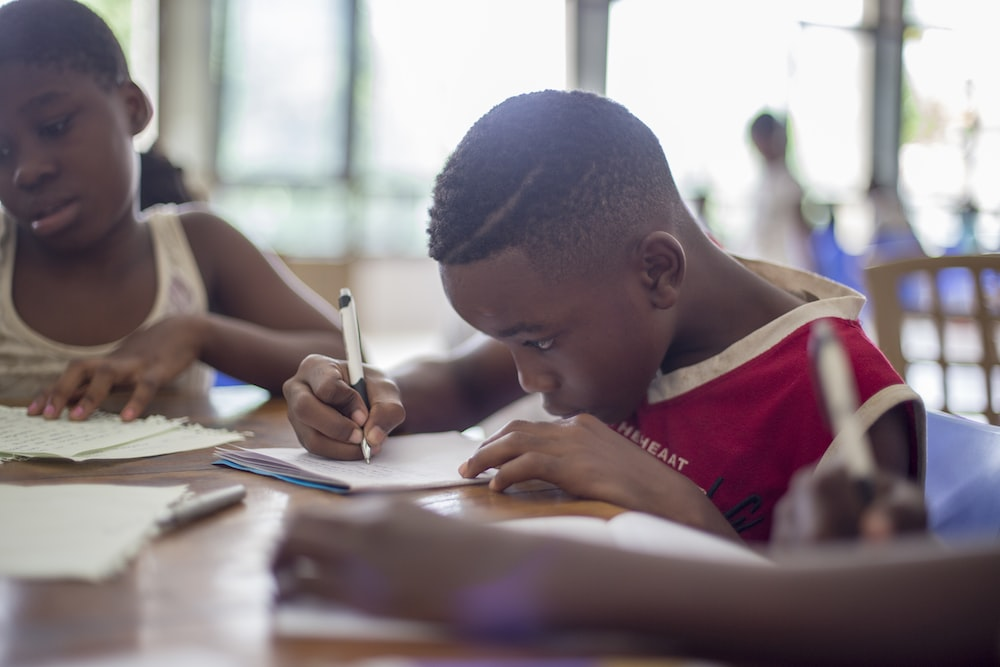
\includegraphics[width=.5\textwidth]{./imgs/img4.jpg}
\caption{Fonte: https://unsplash.com/pt-br/fotografias/O5EMzfdxedg. Acesso em 21/02/2023.}
\end{figure}

\conteudo{Existem diversas maneiras de nos expressarmos textualmente. Podemos, por
exemplo, escrever uma matéria jornalística para informar o público a
respeito de temas importantes para a sociedade. Podemos, ainda, escrever
narrativas e peças de teatro com aprendizados necessários para o
desenvolvimento do ser humano.

É importante reconhecermos os diferentes tipos de textos que encontramos
em nosso dia a dia. Para tanto, devemos localizar as características
específicas de cada forma de expressão. Comecemos pela narrativa. O
principal traço de um texto desse tipo é o desenvolvimento de uma hisstória com personagens, espaço e tempo por meio da intermediação de um narrador.

Para compreendermos algumas dessas características, tomemos como exemplo
o início de uma famosa história infantil.

\begin{quote}
\textbf{Chapeuzinho Vermelho}

Era uma vez uma menina chamada Chapeuzinho Vermelho. Ela morava em uma
casa na floresta com sua mãe.

Certo dia, a mãe de Chapeuzinho lhe fez um pedido:

--- Minha filha, leve esses doces para sua avó! Ela está doente!

A alegre menina respondeu:

--- Mas é claro, mamãe!

Chapeuzinho Vermelho colocou sua capa vermelha e saiu em sua jornada.

Enquanto caminhava pela floresta, Chapeuzinho Vermelho encontrou um lobo
malvado, que perguntou para onde ela estava indo. Chapeuzinho Vermelho
respondeu que estava indo visitar sua avó e mostrou-lhe o caminho.

{[}...{]}.
\end{quote}

A presença de personagens é uma característica que podemos destacar
nesse trecho. Nesse caso específico, encontramos Chapeuzinho Vermelho,
sua mãe e o lobo. Um texto narrativo deverá sempre apresentar
personagens que, em certo sentido, conduzem a história sendo contada,
mas são apresentados por um narrador. Quando aparece, as falas são
introduzidas por um travessão, tal como pode ser observado no trecho.

Os diálogos normalmente são introduzidos por meio de verbos de
enunciação, isto é, verbos que indicam alguma ação relacionada à fala.
Nesse trecho de ``Chapeuzinho Vermelho'', encontramos o verbo ``responder''
antes da resposta de Chapeuzinho. Outros verbos comuns são: ``falar'',
``dizer'', ``afirmar'', ``exclamar'', por exemplo.

Por fim, é necessário percebermos também como uma narrativa sempre
apresenta um narrador, ou seja, uma voz que conta a história. No trecho
reproduzido, é possível percebermos como a narrativa é apresentada
aos leitores por meio de uma voz que parece conhecer todos os fatos a
serem transmitidos.

Semelhante, em alguns aspectos, a uma narrativa, mas diferente em outros, existe o texto dramático, que é aquele escrito para ser encenado. Talvez, você já tenha asssistido a uma peça de teatro no palco. Para aprenderem suas falas
e apresentarem a história em cima do palco, os atores devem ler o texto
dramático, que consiste em uma sequência de diálogos
entre personagens.

Tomemos como exemplo uma história de Chapeuzinho
Vermelho em formato de texto dramático.


\includegraphics[width=.5\textwidth]{./imgs/img5.png}
%\caption{Fonte: https://pixabay.com/pt/vectors/chapeuzinho-vermelho-garota-corrida-156953/. Acesso em 21/02/2023.}

\begin{quote}
Chapeuzinho Vermelho (aproximando-se da cama): Para que esses olhos
tão grandes, vovozinha?

Lobo: São para te enxergar melhor!

Chapeuzinho Vermelho: E para que essas orelhas tão grandes, vovozinha?

Lobo: São para te escutar melhor!
\end{quote}

Percebemos como um texto dramático apresenta os diálogos a serem
decorados pelos atores de uma peça. Ao invés de um travessão, as falas são introduzidas pelos nomes dos personagens envolvidos.

Podemos, ainda, notar a presença da descrição de uma ação a ser realizada, que,
no caso, é a aproximação de Chapeuzinho à cama de sua avó. Essas indicações marcam a ação dos atores no palco. Assim,
constatamos como, em um texto dramático, o desenrolar da história é
apresentado diretamente ao leitor, sem a presença de um narrador.}

\colorsec{Atividades}

\num{1} Como denominamos a voz que apresenta a narrativa aos leitores?

\coment O narrador é que apresenta os fatos de uma história ao leitor.

\linhas{1}

\num{2} Como chamamos os indivíduos que participam de uma narrativa e de um
texto dramático?

\coment{Tanto o texto narrativo quanto o texto dramático contam com a presença de personagens.}

\linhas{1}

\num{3} Em um texto dramático, como a história é apresentada ao leitor?

\coment{Um texto dramático apresenta o diálogo como sua estrutura básica.}

\linhas{1}

\num{4} Assinale V para o que for verdadeiro e F para o que for falso.

\begin{boxlist}
\item Em um texto dramático, não são descritas as ações dos personagens. \coment{F}

\item O verbo ``falar'' pode ser usado para introduzir um diálogo. \coment{V}

\item Um texto dramático sempre apresenta um narrador. \coment{F}

\item Diferentemente do texto dramático, o texto narrativo não é escrito para ser encenado. \coment{V}
\end{boxlist}

Leia o texto e responda às questões 5 e 6.

\begin{quote}
Príncipe (caminhando em direção à torre, gritando): Quem é esta bela
donzela presa no topo da torre?

Rapunzel: Sou eu: Rapunzel! A jovem dos cabelos dourados.
\fonte{Texto escrito para este material.}
\end{quote}

\num{5} Quais são os personagens envolvidos nesse texto?

\linhas{2}
\coment{O texto apresenta os personagens Príncipe e Rapunzel.}

\num{6} Mesmo não se tratando de um texto narrativo, aparece um verbo de enunciação antecedendo a fala do Príncipe. Que verbo é esse?

\linhas{2}
\coment{Foi utilizado o verbo ``gritar''.}

\num{7} Associe as colunas.

\begin{multicols}{2}
(1) Texto narrativo\medskip

(2) Texto dramático

\columnbreak

(\coment{1}) Presença de um narrador.

(\coment{2}) Diálogos introduzidos pelos nomes dos personagens.

(\coment{2}) Ação apresentada diretamente ao leitor.

(\coment{1}) Diálogos introduzidos por um travessão.
\end{multicols}

\num{8} Qual é a diferença fundamental eentre um texto narrativo e um texto dramático?

\linhas{3}
\coment{Em um texto narrativo, a história é contada pelo narrador. Já em um texto
dramático, a ação acontece a partir dos diálogos entre os personagens.}


Leia o texto e responda às questões 9 e 10.

\begin{figure}[htpb!]
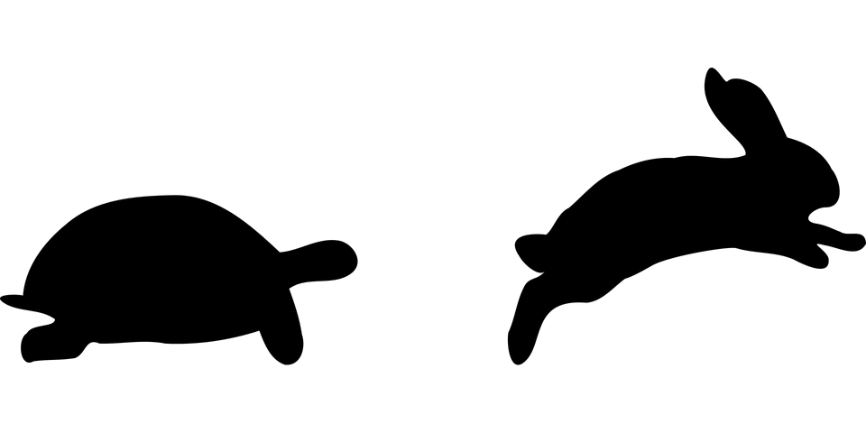
\includegraphics[width=.5\textwidth]{./imgs/img6.png}
\caption{Fonte: https://pixabay.com/pt/vectors/imagens-de-palavras-do-alfabeto-1298865/. Acesso em 21/02/2023.}
\end{figure}

\begin{quote}
Certa vez, uma lebre e uma tartaruga decidiram apostar uma corrida.

A lebre era muito rápida e estava confiante de que venceria. Ela se
deitou para tirar uma soneca enquanto a tartaruga continuava a andar.

No entanto, a tartaruga não desistiu e continuou a se mover em um ritmo
constante. Quando a lebre acordou de sua soneca, viu que a tartaruga
havia quase chegado ao final da corrida.

A lebre correu o mais rápido que pôde para tentar recuperar o atraso,
mas foi tarde demais. A tartaruga cruzou a linha de chegada antes,
vencendo a corrida.
\fonte{Texto escrito para este material.}
\end{quote}

\num{9} Esse texto é uma narrativa ou um drama? Justifique sua resposta.

\linhas{2}
\coment{Trata-se de uma narrativa, pois a ação é apresentada por um narrador, e
não por meio de diálogos.}

\num{10} Quais são os personagens envolvidos no texto?

\linhas{1}
\coment{As personagens são a Lebre e a Tartaruga.}


\colorsec{Treino}

\num{1} Leia o texto.

\begin{quote}
{[}...{]}

--- Errou! --- Interrompeu Camilo, rindo.

--- Não diga isso, Camilo. Se você soubesse como eu tenho andado, por
sua causa. Você sabe; já lhe disse. Não ria de mim, não ria...

Camilo pegou-lhe nas mãos e olhou para ela sério e fixo. Jurou que lhe
queria muito, que os seus sustos pareciam de criança.

{[}...{]}

\fonte{Joaquim Maria Machado de Assis. A Cartomante.
Disponível em: /emph{https://machado.mec.gov.br/obra-completa-lista/item/download/65\_2b8fb9ad43aa37653a58bc2bd56e33aa}. Acesso em: 21 fev. 2023.}
\end{quote}

Os diálogos desse texto narrativo são introduzidos por meio de

\begin{escolha}
\item aspas.

\item travessões.

\item vírgulas.

\item pontos finais.
\end{escolha}

\coment{SAEB: Identificar elementos constitutivos de textos narrativos.
BNCC: EF35LP26 - Ler e compreender, com certa autonomia, narrativas ficcionais
que apresentem cenários e personagens, observando os elementos da
estrutura narrativa: enredo, tempo, espaço, personagens, narrador e a
construção do discurso indireto e discurso direto.

a) Incorreta. Em alguns casos, as aspas indicam falas em textos narrativos, mas não é o que ocorre com o texto em análise.
b) Correta. Os travessões são usados para introduzir as falas dos
personagens.
c) Incorreta. Vírgulas são usadas para separar frases.
d) Incorreta. Pontos finais são usados para finalizar frases.}

\num{2} Leia o texto.

\begin{quote}
{[}...{]}

O estrangeiro disse:

--- Sou dos guerreiros brancos, que levantaram a taba nas margens do
Jaguaribe, perto do mar, onde habitam os pitiguaras, inimigos de tua
nação. Meu nome é Martim, que na tua língua diz como filho de guerreiro;
meu sangue, o do grande povo que primeiro viu as terras de tua pátria.

{[}...{]}.

\fonte{José de Alencar. Iracema. Disponível em: \emph{http://objdigital.bn.br/Acervo\_Digital/Livros\_eletronicos/iracema.pdf}. Acesso em: 21 fev. 2023.}
\end{quote}

O verbo de enunciação utilizado para introduzir a fala do personagem indica que ele

\begin{escolha}
\item pronunciou a fala sem nenhuma forma de expressão específica.

\item gritou aquilo que pretendia pronunciar para seu interlocutor.

\item susurrou para seu interlocutor, mesmo correndo o risco de não ser ouvido.

\item pronunciou a fala indicada nas costas de seu interlocutor.
\end{escolha}

\coment{SAEB: Analisar os efeitos de sentido de verbos de enunciação.
BNCC: EF05LP09 - Ler e compreender, com autonomia, textos instrucionais de
regras de jogo, dentre outros gêneros do campo da vida cotidiana, de
acordo com as convenções do gênero e considerando a situação
comunicativa e a finalidade do texto.

a) Correta. O verbo ``dizer'' demarca uma neutralidade na forma de pronunciar a fala.
b) Incorreta. Não há indicação de que o personagem gritou.
c) Incorreta. Não há indicação de que o personagem sussurrou.
d) Incorreta. Não há indicação no texto da posição do personagem que fala ou da posição de seu interlocutor.}

\num{3} Leia o texto.

\begin{quote}
{[}...{]}

BARÃO (à porta) --- Perdão, minha senhora; eu trazia um livro há
pouco...

D. HELENA (com o livro na mão) --- Será este?

BARÃO (caminhando para ela) --- Justamente.

D. HELENA --- Escrito em sueco, penso eu...

BARÃO --- Em sueco.

{[}...{]}.
\end{quote}

\fonte{Joaquim Maria Machado de Assis. Lição de Botânica. Disponível em: \emph{https://machado.mec.gov.br/obra-completa-lista/item/download/65\_2b8fb9ad43aa37653a58bc2bd56e33aa}. Acesso em: 21 fev. 2023.}

A informação ``caminhando para ela'', entre parênteses, indica
\begin{escolha}
\item uma parte do narrador.

\item uma marcação do cenário.

\item o início de uma fala.

\item uma ação do personagem.
\end{escolha}

\coment{SAEB: Identificar as marcas de organização de textos dramáticos.
BNCC: EF35LP24 - Identificar funções do texto dramático (escrito para ser
encenado) e sua organização por meio de diálogos entre personagens e
marcadores das falas das personagens e de cena.

a) Incorreta. Trata-se de um texto dramático; portanto não há narrador.
b) Incorreta. A informação não se relaciona com o cenário da peça.
c) Incorreta. A indicação entre parênteses, apesar de aparecer antes da fala, após a nomeação do personagem, não abre uma fala.
d) Correta. A indicação marca que o personagem fala enquanto caminha em direção à outra personagem.}

\chapter{3. O gênero notícia}

\coment{Neste módulo, estudaremos o gênero textual notícia. Você deve
examinar os traços associados a esse gênero com os alunos,
destacando sua natureza informativa. Também exploraremos algumas regras
de pontuação da língua portuguesa a partir das notícias apresentadas.\\
Habilidades da BNCC: EF35LP16 e EF05LP14.}

\colorsec{Habilidades do SAEB}

\begin{itemize}
\item Analisar elementos constitutivos de gêneros textuais diversos.

\item Reconhecer os usos da pontuação.

\item Analisar os efeitos de sentido decorrentes do uso da pontuação.
\end{itemize}

\begin{figure}[htpb!]
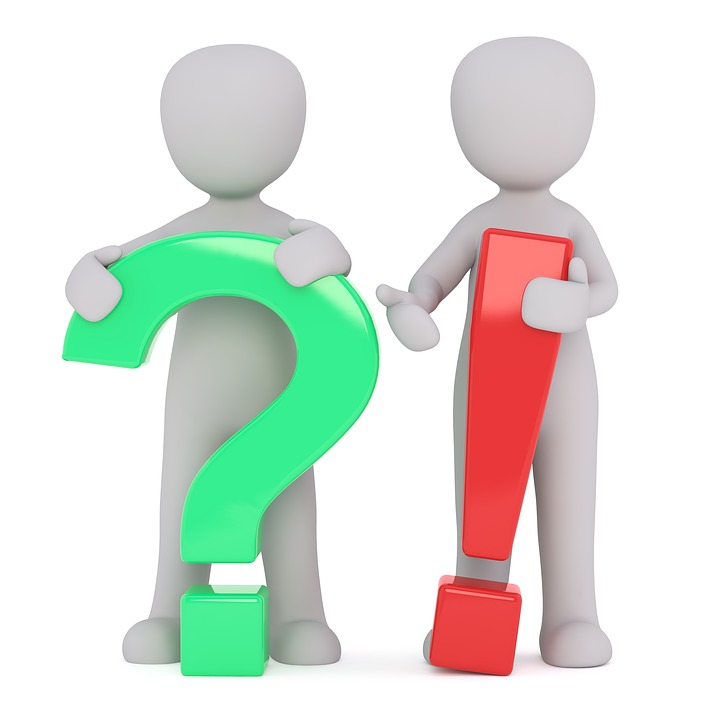
\includegraphics[width=.5\textwidth]{./imgs/img7.jpg}
\caption{Fonte: https://pixabay.com/pt/illustrations/ponto-de-interroga\%c3\%a7\%c3\%a3o-pergunta-ajuda-2314115/. Acesso em 21/02/2023.}
\end{figure}

\conteudo{Cotidianamente, entramos em contato com muitos gêneros textuais
diferentes. Cada texto possui características próprias
relacionadas ao assunto explorado e ao público que pretende atingir.
Devemos conhecer esses traços para identificarmos as muitas formas de
nos expressarmos. Para exemplificarmos esse processo, tomemos como
exemplo um gênero muito comum em nosso dia a dia.

Uma excelente maneira de nos mantermos informados a respeito do mundo se
dá por meio da leitura de notícias veiculadas, por exemplo, em jornais, revistas ou sites de
internet. De modo geral, esse gênero trata de fatos recentes de alguma
relevância para a sociedade. Ao consumirmos uma notícia, devemos
nos atentar para algumas de suas características principais a fim de
absorvermos todo o seu conteúdo.

Para identificar os traços estilísticos de uma notícia, leia o trecho
a seguir.

\begin{quote}
\textbf{Brasileiros estão entre os que mais receberam vistos norte-americanos}
\textit{País ficou atrás apenas de México e China em 2022}

Pesquisa da AG Immigration – escritório de advocacia imigratória com sede em Washington – mostra que os brasileiros ocuparam o terceiro lugar no ranking dos que mais receberam vistos norte-americanos em 2022. Ao todo, foram 815.842 emissões de 80 tipos diferentes de permissões, alta de 618,8\% em relação ao registrado no ano anterior (113.505). Em comparação com 2018 (640.998), nos níveis de antes da pandemia de covid-19, o aumento foi de 26,4\%.

O Brasil ficou atrás apenas do México (1,9 milhão) e da China (1 milhão), e bem à frente da Argentina, quarta colocada, com 259 mil vistos recebidos.

O levantamento foi feito com base em dados oficiais do Departamento de Estado norte-americano, de janeiro a dezembro de 2022. {[}...{]}.

\fonte{Ana Cristina Campos. Brasileiros estão entre os que mais receberam vistos norte-americanos. Agência Brasil. Disponível em: \emph{https://agenciabrasil.ebc.com.br/internacional/noticia/2023-03/brasileiros-estao-entre-os-que-mais-receberam-vistos-norte-americanos}. Acesso em: 23 mar. 2023.}
\end{quote}

Em primeiro lugar, é possível identificar o título da notícia: ``Brasileiros estão entre os que mais receberam vistos norte-americanos''. Nos locais em que costumam ser veiculadas as notícias, o título geralmente ocupa o
centro da página e apresenta uma fonte maior, em destaque. Dessa forma,
o leitor será capaz de compreender o assunto da notícia.

Logo em seguida, logo abaixo do título, aparece o subtítulo, que amplia as informações do título e, no caso dessa notícia, destaca um ponto relevante presente no corpo do texto.

Então, inicia-se o texto da notícia em si. O primeiro parágrafo de uma notícia, chamado de \textbf{lide}, condensa todas as informações a serem pormenorizadas no corpo do texto, que se inicia no próximo parágrafo.

Algo que devemos ter mente ao lermos o texto de uma notícia é a natureza
expressiva utilizada por seu autor. É possível transmitir informações
aos leitores, não somente por meio de palavras, mas também sinais de
pontuação. No texto acima, por exemplo, encontramos o uso recorrente de
vírgulas e pontos finais, por exemplo. Enquanto as vírgulas são usadas
para separar diferentes frases e organizar os elementos que as compõem, o
ponto final marca o final de um enunciado.}

\colorsec{Atividades}

\num{1} Como podemos diferenciar os diversos gêneros textuais que
encontramos todos os dias?

\linhas{4}
\coment{Devemos conhecer as características específicas de cada gênero textual, bem como o meio em que circulam e o objetivo a que se propõem.}


\num{2} Em geral, do que trata uma notícia?

\linhas{2}
\coment{Uma notícia trata de fatos recentes relevantes para a sociedade.}

\num{3} Como se chama a parte de uma notícia que surge ao centro da página
em uma fonte maior?

\linhas{1}
\coment{Trata-se do título da notícia, que também pode ser denominado de manchete.}

\num{4} Qual é a função do texto inserido logo após o título de uma notícia? Como ele se chama?

\linhas{4}
\coment{Trata-se do subtítulo, que cumpre funções como ampliar as informações do título, resumir o conteúdo da notícia ao leitor ou, ainda, destacar um ponto importante do corpo do texto.}

\num{5} Pensando no fluxo de leitura de notícias, tente refletir sobre a importância do lide e explique por que o primeiro parágrafo pode ser importante nesse sentido.

\linhas{6}
\coment{Alguns leitores podem se interessar por ler muitas notícias seguidamente, e,
nesse sentido, a condensação das informações importantes sobre um fato em um mesmo
parágrafo (o primeiro) pode ajudar o leitor a terminar a leitura de forma mais ágil,
de modo que se parta para os próximos parágrafos caso sinta necessidade de ter detalhes
sobre um aspecto.}

\num{6} Assinale V para o que for verdadeiro e F para o que for falso.

\begin{boxlist}
\item Uma notícia não costuma apresentar um título. \coment{F}

\item O principal assunto da notícia não costuma aparecer em seu título. \coment{F}

\item O principal intuito de uma notícia é informar o leitor. \coment{V}

\item Uma notícia deve expor ao leitor diferentes informações sobre \coment{V}
determinado tema.
\end{boxlist}

\num{7} Associe as colunas.

\begin{multicols}{2}
(1) Ponto final.\medskip

(2) Vírgula.\medskip

(3) Interrogação.\medskip

(4) Exclamação.

\columnbreak

(\coment{3}) Sinal de pontuação que serve para indicar uma pergunta. 

(\coment{2}) Sinal de pontuação que é utilizado para separar frases. 

(\coment{1}) Sinal de pontuação que é colocado ao final das frases. 

(\coment{4}) Sinal de pontuação que é usado para destacar informações. 
\end{multicols}

Leia o texto a seguir e responda às questões de 8 a 10.

\begin{quote}
\textbf{Quaoar, espécie de primo de Platão, tem anel}
\textit{A descoberta desafia a principal teoria de formação de anéis}

Quaoar é um dos grandes objetos de grande porte que orbita além de Netuno.
Recentemente, pesquisadores de vários países descobriram que Quaoar tem um
anel, e isso sugere que essa estrutura deve ser bem mais comum do que se
pensava até então. Com isso, a compreensão sobre a formação de um anel
foi colocada em xeque.

\fonte{Fonte de pesquisa: Salvador Nogueira. Brasileiros descobrem anel em Quaoar,
'primo' de Plutão. Folha de S.Paulo. Disponível em: \emph{https://www1.folha.uol.com.br/ciencia/2023/02/brasileiros-descobrem-anel-em-quaoar-primo-de-plutao.shtml}. Acesso em: 23 mar. 2023.}
\end{quote}

\num{8} Com base nesse primeiro parágrafo da notícia, depreenda qual é o assunto tratado.

\linhas{3}
\coment{A notícia trata da descoberta de um anel ao redor de um corpo celeste longínquo chamado Quaoar.}


\num{9} O título da notícia é totalmente claro, para qualquer leitor, com relação ao assunto tratado?

\linhas{3}
\coment{Pode-se perceber que, sobretudo para um leitor leigo, o assunto da notícia só fica totalmente claro no primeiro parágrafo da notícia.}


\num{10} Quais são os sinais de pontuação encontrados no texto e quais são
suas funções?

\linhas{3}
\coment{O texto apresenta vírgulas e pontos finais. Esses sinais são utilizados
para separar frases e indicar o fim de uma sentença, respectivamente.}


\colorsec{Treino}

\num{1} Leia o texto.

\begin{figure}[htpb!]
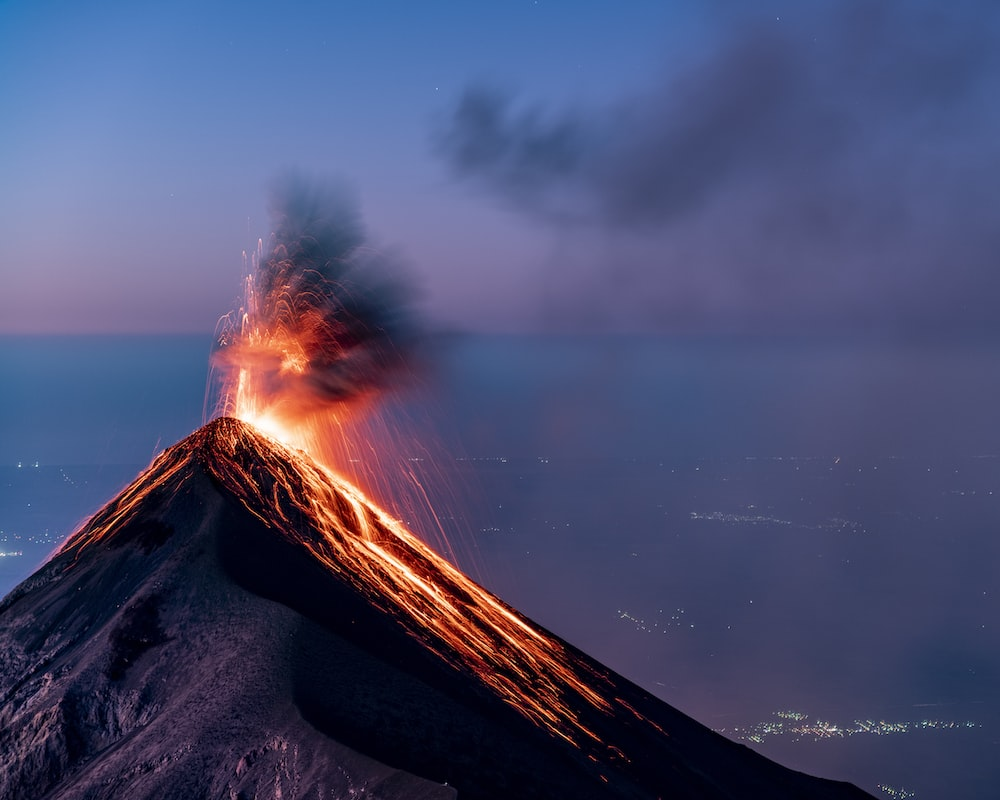
\includegraphics[width=.5\textwidth]{./imgs/img9.jpg}
\caption{Fonte: https://unsplash.com/pt-br/fotografias/tLxGw\_ITs7k. Acesso em 21/03/2022.}
\end{figure}

\begin{quote}
\textbf{Maior vulcão ativo do mundo entra em erupção no Havaí}

O maior vulcão ativo do mundo, que fica no Havaí, entrou em erupção pela primeira vez em 40 anos. Localizado no Parque Nacional dos Vulcões, o Mauna Loa cobre metade da Ilha do país e se eleva há mais de quatro mil metros do nível do mar.

O fluxo de lava está localizado principalmente no cume, mas os moradores foram colocados em alerta. No entanto, nenhuma ordem para deixar o local foi emitida, pois as autoridades acham improvável que as áreas povoadas sejam afetadas nesta fase. Um aviso de queda de cinzas chegou a ser emitido, mas já foi suspenso.

De acordo com o Serviço Geológico dos Estados Unidos, o Mauna Loa entrou em erupção 33 vezes desde 1843. A última foi em 1984, quando as lavas chegaram a atingir a cidade de Hilo, a mais populosa da ilha.

\fonte{Repórter Brasil Tarde. Maior vulcão ativo do mundo entra em erupção no Havaí. Disponível em: \emph{https://tvbrasil.ebc.com.br/reporter-brasil-tarde/2022/11/maior-vulcao-ativo-do-mundo-entra-em-erupcao-no-havai}. Acesso em: 23 mar. 2023.}
\end{quote}

O uso do presente do indicativo (``entra'') no título do texto

\begin{escolha}
\item aproxima do leitor o fato ocorrido e noticiado.

\item cria uma distância temporal entre o fato e a notícia.

\item estabelece que o fato noticiado ainda está para acontecer.

\item demonstra que o fato ocorre no momento da publicação da notícia.
\end{escolha}

\coment{SAEB: Analisar elementos constitutivos de gêneros textuais diversos.
BNCC: EF35LP16 - Identificar e reproduzir, em notícias, manchetes, lides
e corpo de notícias simples para público infantil e cartas de reclamação
(revista infantil), digitais ou impressos, a formatação e diagramação
específica de cada um desses gêneros, inclusive em suas versões orais.

a) Correta. É comum, em notícias, o uso do presente do indicativo para noticiar fatos já ocorridos, o que aproxima o fato do leitor.
b) Incorreta. Pelo contrário, cria-se uma aproximação temporal.
c) Incorreta. O presente do indicativo, nesses casos, substitui a forma no pretérito.
d) Incorreta. O fato ocorreu antes do momento da publicação da notícia.}

\num{2} Leia o texto.

\begin{quote}
\textbf{Novo mapa da Via Láctea revela mais de 3,3 bilhões de objetos e
detalhes inéditos da nossa galáxia}
\textit{Catálogo pode ser considerado o maior do tipo até então}

Uma nova imagem com detalhes sem precedentes da Via Láctea foi lançada
nesta quinta-feira (19) para marcar a segunda fase de uma das maiores
pesquisas de rastreio da galáxia da qual o nosso Sistema Solar faz parte
{[}...{]}.

Como resultado do levantamento gigantesco, que levou dois anos para ser
concluído, cerca de 3,32 bilhões de objetos foram identificados, o que
pode ser considerado o maior catálogo do tipo até então.

{[}...{]}
\fonte{Roberto Peixoto. Novo mapa da Via Láctea revela mais de 3,3 bilhões de objetos e detalhes inéditos da nossa galáxia. G1. Disponível em: \emph{https://g1.globo.com/ciencia/noticia/2023/01/19/novo-mapa-da-via-lactea-revela-mais-de-33-bilhoes-de-objetos-e-detalhes-ineditos-da-nossa-galaxia.ghtml}. Acesso em: 23 mar. 2023.}
\end{quote}

Uma marca temporal presente nessa notícia revela que o fato noticiado é

\begin{escolha}
\item recente.

\item antigo.

\item ultrapasado.

\item futuro.
\end{escolha}

\coment{SAEB: Analisar elementos constitutivos de gêneros textuais diversos.
BNCC: EF35LP16 - Identificar e reproduzir, em notícias, manchetes, lides
e corpo de notícias simples para público infantil e cartas de reclamação
(revista infantil), digitais ou impressos, a formatação e diagramação
específica de cada um desses gêneros, inclusive em suas versões orais.

a) Correta. A marca ``nesta quinta-feira (19)'' demonstra que se trata de um fato que, na época de publicação da notícia, era recente.
b) Incorreta. Demonstra-se, no texto, que o acontecimento é recente.
c) Incorreta. Não há um juízo de valor quanto ao fato.
d) Incorreta. Está claro no texto que o fato é passado.}

\num{3} Leia o texto.

\begin{quote}
\textbf{Mais energia do que o Sol? Cientistas devem revelar 'grande
avanço científico'}

O Departamento de Energia dos Estados Unidos afirmou no domingo que
anunciará durante a semana um "grande avanço científico", depois que
vários meios de comunicação informaram que um laboratório federal
alcançou recentemente um marco importante na pesquisa da fusão nuclear.

{[}...{]}.

\fonte{TILT. Mais energia do que o Sol? Cientistas devem revelar 'grande
avanço científico'. Disponível em: \emph{https://www.uol.com.br/tilt/noticias/afp/2022/12/12/mais-energia-do-que-o-sol-cientistas-irao-revelar-grande-marco-em-fusao-nuclear.htm}. Acesso em: 21 mar. 2023.}
\end{quote}

O ponto de interrogação é empregado no título da notícia para

\begin{escolha}
\item indicar uma pergunta.

\item destacar o tema a ser discutido.

\item dividir duas frases.

\item indicar o final do texto.
\end{escolha}

\coment{SAEB: Analisar os efeitos de sentido decorrentes do uso da pontuação.
BNCC: EF05LP04 - Diferenciar, na leitura de textos, vírgula, ponto e
vírgula, dois-pontos e reconhecer, na leitura de textos, o efeito de
sentido que decorre do uso de reticências, aspas, parênteses.

a) Correta. O ponto de interrogação é usado para indicar uma pergunta.
b) Incorreta. O ponto de exclamação é usado para destacar uma
informação.
c) Incorreta. A vírgula é usada para dividir duas frases.
d) Incorreta. O final de um texto é indicado por um ponto final.}

\chapter{4. Argumentação e persuasão}

\coment{Os alunos serão expostos a textos argumentativos neste módulo. O
professor deverá analisar as características do gênero a fim de
demonstrar como um argumento convincente é construído. Além disso, a
partir da leitura de imagens serão também estudadas as possibilidades
multissemióticas implícitas no processo de argumentação.\\
Habilidade BNCC: EF05LP20.}

\colorsec{Habilidades SAEB}

\begin{itemize}
\item Analisar o uso de recursos de persuasão em textos verbais e/ou
multimodais.

\item Analisar os efeitos de sentido de recursos multissemióticos em textos
que circulam em diferentes suportes.

\item Julgar a eficácia de argumentos em textos.
\end{itemize}

\begin{figure}[htpb!]
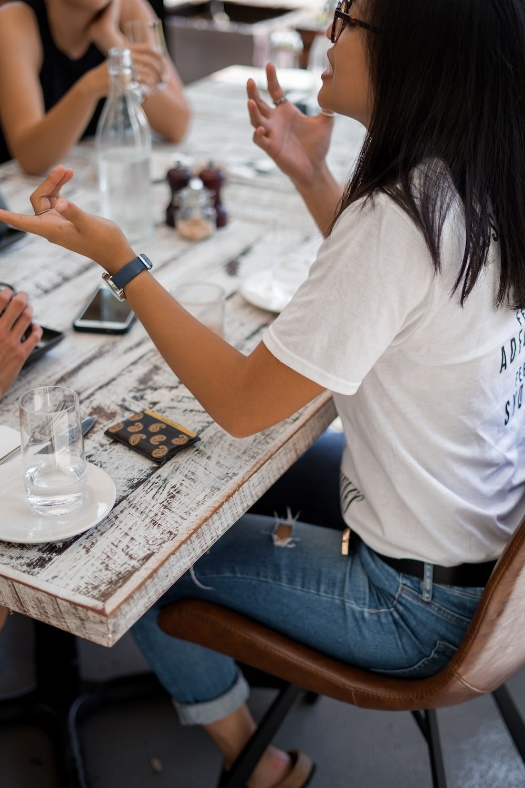
\includegraphics[width=.5\textwidth]{./imgs/img10.jpg}
\caption{Fonte: https://unsplash.com/pt-br/fotografias/wXJViXxHP44. Acesso em 20/02/2023.}
\end{figure}

\conteudo{No módulo anterior, estudamos o gênero notícia, um tipo de texto focado
na transmissão de informações. É importante, todavia, destacarmos outras
possibilidades textuais que buscam criar efeitos diversos nos leitores.
É possível, por exemplo, encontrarmos textos que tentam convencer o
público da validade de um ponto de vista ou ação. Denominamos esse texto
de ``argumentativo''.

Ao analisarmos esse gênero, é importante termos em mente dois aspectos
importantes: o argumento de que o autor está tentando convencer os
leitores e as estratégias utilizadas para atingir esse objetivo. Leiamos
o texto a seguir para exemplificarmos esses traços:

\begin{quote}
\textbf{A Turminha está em campanha contra a dengue}

A Turminha do MPF anda preocupada com a dengue. Também não é para
menos: a Sol foi picada pelo mosquito e ficou dodói. Depois de vários
dias de repouso, tomando muito líquido, agora já está bem.

A Malu, preocupada com a amiga doente, ficou indignada com pessoas que
deixam água parada e alertou os amigos da Turminha para chamarem a
defesa civil quando souberem de algum lote vazio onde haja foco de
dengue. Na rua do Rafinha houve um surto de dengue e muitas pessoas
ficaram doentes. Ele deu dicas sobre os cuidados com as piscinas e com
objetos que acumulam água, como pneus, garrafas, tampinhas etc.

{[}...{]}.

\fonte{Fonte:
https://turminha.mpf.mp.br/explore/direitos-das-criancas/saude/dicas-de-saude.
Acesso em 21/02/2023.}
\end{quote}

Consegue identificar o argumento construído acima? Trata-se de um texto
escrito com o intuito de expor os perigos da dengue e de convencer as
crianças da necessidade de combatermos o mosquito Aedes Aegypti. Para
isso, o autor utiliza o exemplo da garotinha Sol, que contraiu a doença
e teve de passar alguns dias de repouso até se curar. Assim, para se
criar um argumento convincente, é importante exemplificar situações
relacionados ao assunto explorado.

Ao construirmos um argumento, é necessário explicarmos o que o leitor
deve fazer para atingir o objetivo exposto em nosso texto. No caso
específico do combate à dengue, foram enumeradas, no trecho acima,
atitudes a serem tomadas a fim de impedir a proliferação do mosquito da
dengue -- chamar a Defesa Civil, não deixar água parada em pneus etc.
Dessa forma, podemos dizer que a argumentação depende de ações
explicadas objetivamente.

Um texto argumentativo pode também ser construído a partir de outras
formas de expressão que não a da escrita. A utilização de imagens é uma
estratégia eficiente e chamativa para fortalecer um argumento. Em um
texto sobre a dengue, é possível, por exemplo, encontrarmos um pôster
que estimule o combate ao mosquito. Veja a imagem a seguir:

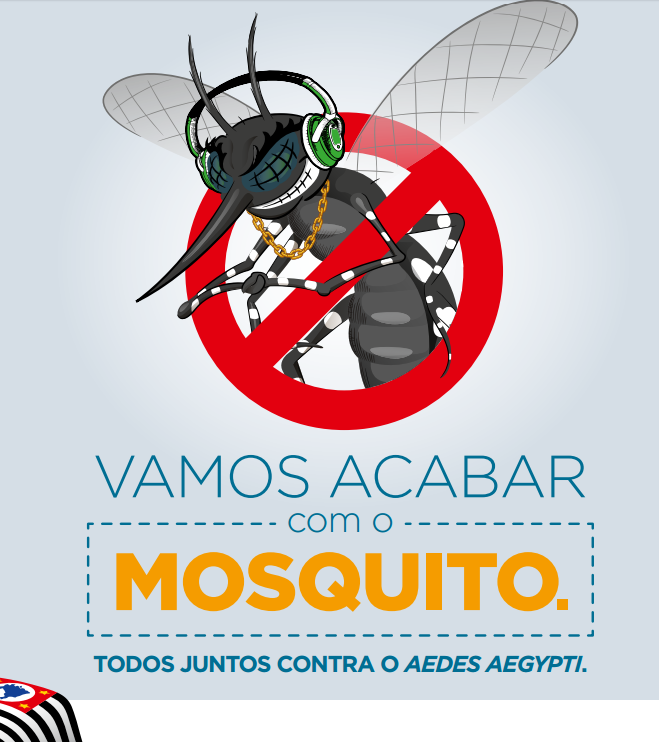
\includegraphics[width=.5\textwidth]{./imgs/img11.png}
%\caption{Fonte: https://www.saopaulo.sp.gov.br/tag/dengue/. Acesso em 21/02/2023.}

Assim, é possível percebermos como um texto argumentativo lança mão de
diferentes estratégias para atingir seus objetivos, até mesmo de
artifícios visuais. No cartaz acima, o desenho do mosquito dentro do
símbolo associado a proibição fortalece o argumento a ser desenvolvido.
De maneira chamativa, a necessidade de tomarmos atitudes diretas conta o
Aedes Aegypti é salientada.

Após a leitura de um texto argumentativo, o leitor poderá julgar se as
estratégias transmitidas foram eficientes, isto é, se o texto foi
convincente ou não. A eficácia de um argumento está diretamente
relacionada à qualidade dos exemplos e ações apresentados. No texto de
combate à dengue, podemos dizer que o autor conseguiu desenvolver uma
ideia convincente, já que ofereceu exemplos e ações capazes de
solucionar o problema exposto.}

\colorsec{Atividades}

\num{1} Como denominamos o gênero textual utilizado para convencer o leitor
de algo?


\linhas{1}
\coment{Trata-se do texto argumentativo.}

\num{2} Quais são os dois elementos principais desse tipo de texto?

\linhas{2}
\coment{Um texto argumentativo é constituído por argumentos e estratégias.}


\num{3} Assinale V para verdadeiro e F para falso.

\begin{boxlist}
\item Um texto argumentativo não deve citar exemplos. \coment{F}

\item Um texto argumentativo não deve convencer o leitor a respeito de 
um ponto de vista. \coment{F}

\item Um texto argumentativo deve apresentar ações a serem realizadas pelo leitor. \coment{V} 

\item Um texto argumentativo só deve ser constituído por palavras. \coment{F}
\end{boxlist}

\num{4} Após a leitura de um texto argumentativo, como podemos julgar os argumentos apresentados?


\linhas{2}
\coment{Devemos verificar se os argumentos apresentados foram convincentes.}

\num{5} Complete a frase a seguir:

Além da escrita, um texto argumentativo pode apresentar \preencher.

\coment{Imagens.}

\num{6} Leia o texto a seguir e responda às perguntas:

\begin{quote}
\textbf{SP contra o novo coronavírus}

{[}...{]}

Lave as mãos

\begin{figure}[htpb!]
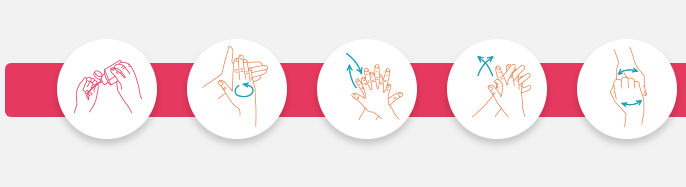
\includegraphics[width=.5\textwidth]{./imgs/img12.png}
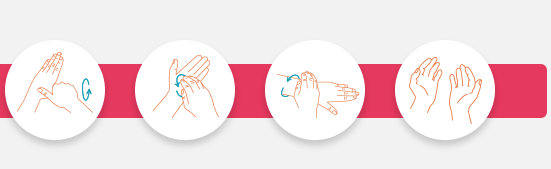
\includegraphics[width=.5\textwidth]{./imgs/img13.png}
\end{figure}

A principal recomendação é higienizar as mãos. São cuidados simples,
mas importantes e que devem ser frequentes para prevenir doenças
contagiosas.

Higienize as mãos frequentemente com água e sabão ou use antisséptico de
mãos à base de álcool gel 70\% {[}...{]}.

{[}...{]}

Ao tossir e espirrar

\begin{figure}[htpb!]

\includegraphics[width=.5\textwidth]{./imgs/img14.png}
\end{figure}

Cubra a boca e o nariz. Use os braços ou lenço descartável. Evite usar
as mãos. E, se usar, lembre-se de higienizá-las.

{[}...{]}.

\fonte{Fonte: https://www.saopaulo.sp.gov.br/coronavirus/.
Acesso em 21/02/2023.}
\end{quote}

\begin{escolha}
\item Qual é o principal argumento encontrado no texto acima?

\linhas{3}
\coment{O texto procura convencer o leitor da necessidade de combatermos a
transmissão do coronavírus a partir da higienização das mãos e dos
cuidados a serem observados ao tossirmos e espirrarmos.}


\item Procure no texto duas ações a serem realizadas contra o
coronavírus.

\linhas{2}
\coment{De acordo com o texto, devemos higienizar as mãos constantemente e
cobrir a boca ao tossir ou espirrar.}


\item O trecho reproduzido acima apresenta duas imagens. Como elas se
relacionam aos argumentos apresentados?

\linhas{2}
\coment{As imagens ensinam os leitores a lavarem as mãos da forma correta e como
devem cobrir a boca ao tossir e espirrar.}
\end{escolha}

\num{7} Que tipo de recursos além da palavra escrita um texto argumentativo
pode apresentar?

\linhas{1}
\coment{Um texto argumentativo pode apresentar, por exemplo, imagens.}


\num{8} Por que é importante que um texto argumentativo traga também esses recursos?

\linhas{2}
\coment{Um texto argumentativo lança mão desse tipo de recurso para fortalecer o
ponto de vista defendido.}


\colorsec{Treino}

\num{1} Leia o texto a seguir e responda à questão:

\begin{quote}
\textbf{Vacina é vida!}

Vacinas salvam vidas, são seguras, não causam doenças e protegem a
comunidade! Segundo a Organização Mundial de Saúde, graças às vacinas
são evitadas, a cada ano, entre 2 e 3 milhões de mortes por doenças
preveníveis. Pensando nisso, o Instituto e a Fundação Butantan, em
parceria com a Sanofi Pasteur e a Secretaria Municipal de Educação de
São Paulo, com o apoio da Secretaria de Estado da Saúde de São Paulo e
da Secretaria Municipal de Saúde de São Paulo, promovem a Campanha ``A
Importância da Vacinação.

{[}...{]}.

\fonte{Fonte: https://campanhavacina.butantan.gov.br/. Acesso
em 21/02/2023.}
\end{quote}

No texto acima, o argumento desenvolvido refere-se

\begin{escolha}
\item às etapas de fabricação das vacinas.

\item aos perigos associados à vacinação.

\item aos números da vacinação contra o coronavírus.

\item à importância da vacinação.
\end{escolha}

\coment{Dificuldade: Fácil.

Saeb: Analisar o uso de recursos de persuasão em textos verbais e/ou
multimodais. BNCC: (EF05LP20) Analisar a validade e força de argumentos
em argumentações sobre produtos de mídia para público infantil (filmes,
desenhos animados, HQs, games etc.), com base em conhecimentos sobre os
mesmos.

a) Incorreta. O texto não faz menção ao processo de fabricação das
vacinas;
b) Incorreta. O texto desenvolve justamente o argumento oposto;
c) Incorreta. O texto não cita uma doença específica;
d) Correta. O texto salienta a importância da vacinação.}

\num{2} Leia o texto a seguir e responda à pergunta:

\begin{quote}
As vacinas são seguras?

As vacinas são muito seguras. É muito mais provável que sua criança seja
prejudicada por uma doença evitável por vacina do que por uma vacina.
Todas as vacinas passam por rigorosos testes de segurança, incluindo
estudos clínicos, antes de ser aprovadas para o público. Os países só
registram e distribuem vacinas que atendam a rigorosos padrões de
qualidade e segurança.

{[}...{]}.

\fonte{Fonte:
https://www.unicef.org/brazil/vacinas-perguntas-e-respostas.
Acesso em 21/02/2023.}
\end{quote}

De acordo com o texto, um argumento para a vacinação é

\begin{escolha}
\item os rigorosos testes de segurança.

\item a quantidade de doenças que surgiu no último ano.

\item o baixo número de testes clínicos disponíveis.

\item a baixa probabilidade de uma criança ficar doente.
\end{escolha}

\coment{Dificuldade: Média.

Saeb: Julgar a eficácia de argumentos em textos. BNCC: (EF05LP20)
Analisar a validade e força de argumentos em argumentações sobre
produtos de mídia para público infantil (filmes, desenhos animados, HQs,
games etc.), com base em conhecimentos sobre os mesmos.

a) Correta. O texto menciona os testes pelos quais uma vacina deve
passar;
b) Incorreta. O texto menciona doenças, mas não as situa no ano passado;
c) Incorreta. O texto diz exatamente o contrário;
d) Incorreta. O texto menciona a possibilidade de uma criança ficar
doente caso não seja vacinada.}

\num{3} Analise a imagem abaixo e responda à pergunta:

\begin{figure}[htpb!]

\includegraphics[width=.5\textwidth]{./imgs/img15.png}
\caption{Fonte: http://www.fundacaocultural.ba.gov.br/2020/03/14210/Governo-do-Estado-anuncia-medidas-para-o-enfrentamento-ao-novo-coronavirus-Covid-19-na-Bahia.html. Acesso em 21/02/2023.}
\end{figure}

De acordo com o cartaz, para combater o coronavírus devemos

\begin{escolha}
\item estimular a vacinação.

\item cumprimentar os colegas com um aperto de mão.

\item higienizar nossas mãos.

\item evitar aglomerações.
\end{escolha}

\coment{Dificuldade: Difícil.

Saeb: Analisar os efeitos de sentido de recursos multissemióticos em
textos que circulam em diferentes suportes. BNCC: (EF05LP20) Analisar a
validade e força de argumentos em argumentações sobre produtos de mídia
para público infantil (filmes, desenhos animados, HQs, games etc.), com
base em conhecimentos sobre os mesmos.

a) Incorreta. A imagem não faz referência à vacinação;
b) Incorreta. Embora a imagem apresente a imagem de duas mãos, não há
referência a cumprimentos;
c) Correta. A imagemapresenta a imagem de duas mãos sendo higienizadas;
d) Incorreta. A imagem não faz referência a aglomerações.}

\chapter{5. Introdução à Poesia}

\coment{Habilidades BNCC: EF35LP27 e EF35LP31.}

\colorsec{Habilidades SAEB}

\begin{itemize}
\item Reconhecer diferentes modos de organização composicional de textos em
versos.

\item Analisar a construção de sentidos de textos em versos com base em seus
elementos constitutivos.
\end{itemize}

\begin{figure}[htpb!]

\includegraphics[width=.5\textwidth]{./imgs/img16.jpg}
\caption{Fonte: https://unsplash.com/pt-br/fotografias/PC-8bIgAVQg. Acesso em 21/03/2023.}
\end{figure}

\conteudo{Após estudarmos alguns gêneros textuais escritos em prosa, passemos
agora a uma modalidade artística diferente. A poesia é uma das formas
mais antigas da literatura. Ela permite que as palavras sejam arranjadas
de maneira criativa, impondo um ritmo e uma sonoridade e evocando
diferentes sensações nos leitores. Ela pode ser encontrada em várias
formas, como sonetos, haicais, poemas épicos etc.

Por meio da poesia, os escritores conseguem capturar o mundo ao seu
redor e expressar suas emoções mais profundas. Trata-se de um gênero
baseado em uma visão individual transformada em forma literária. Em
outras palavras, a poesia se baseia em sentimentos que são transmitidos
ao leitor com o uso expressivo das palavras. Por esse motivo, ela tem
sido valorizada e apreciada ao longo dos séculos.

Cada linha de um poema é denominada verso. Essa seria a unidade básica
do texto. É a partir do verso que apreendemos as imagens e os
sentimentos expostos pelo poeta. Por sua vez, cada conjunto de versos é
denominado estrofe. É justamente a totalidade dessas estrofes que vai
constituir o poema.

Dentro de cada estrofe, os versos normalmente são agrupados a partir de
um mesmo eixo temático. Ao unirmos o conteúdo de cada parte do poema,
extraímos, então, seu sentido geral. Analisemos o exemplo a seguir,
procurando destacar as características únicas do gênero. Perceba como,
em um poema, as linhas não ocupam uma linha inteira:

\begin{quote}
\textbf{Prece}

Senhor, a noite veio e a alma é vil.\\
Tanta foi a tormenta e a vontade!\\
Restam-nos hoje, no silêncio hostil,\\
O mar universal e a saudade.

Mas a chama, que a vida em nós criou,\\
Se ainda há vida ainda não é finda.\\
O frio morto em cinzas a ocultou:\\
A mão do vento pode erguê-la ainda.\\

Dá o sopro, a aragem --- ou desgraça ou ânsia ---,\\
Com que a chama do esforço se remoça,\\
E outra vez conquistemos a Distância ---\\
Do mar ou outra, mas que seja nossa!

\fonte{PESSOA, Fernando. Prece. In: \emph{Mensagem.} São Paulo: Hedra, 2007.}
\end{quote}

Glossário:

Ânsia: vontade\\
Aragem: oportunidade\\
Finda: terminada\\
Hostil: desfavorável\\
Remoçar: rejuvenescer\\
Tormenta: tempestade\\
Vil: desprezível

No poema de Fernando Pessoa reproduzido acima, temos três estrofes, cada
uma com quatro versos. Tal como já foi dito, é possível observarmos um
mesmo assunto sendo desenvolvido em cada uma delas. Na primeira estrofe,
o poeta fala sobre a tristeza trazida pela noite. Já na segunda e na
terceira, é mencionada uma chama capaz de manter a esperança e a vida
acesas. Desse modo, ao lermos uma estrofe após a outra, conseguimos
extrair o sentido do poema como um todo, relacionando suas diferentes
partes.

Devemos destacar também o fato de muitos poemas apresentarem rimas. Elas
consistem na repetição sonora de uma ou mais palavras no final de dois
ou mais versos consecutivos. A função das rimas pode ser diversa:
estabelecer um padrão sonoro, criar musicalidade e ritmo, intensificar a
expressividade, entre outros. Na primeira estrofe do poema de Fernando
Pessoa, encontramos rimas entre as palavras vil/hostil e
vontade/saudade. Dessa forma, percebemos como esse artifício é usado
para criar um sentido de musicalidade que estimula a declamação do
poema, ou seja, sua leitura em voz alta.}

\colorsec{Atividades}

\num{1} Como as palavras são organizadas no gênero poesia?

\linhas{2}
\coment{As palavras são arranjadas de forma criativa, impondo uma sonoridade e
um ritmo.}

\num{2} Qual é o principal objetivo de um poeta ao escrever um poema?

\linhas{2}
\coment{O poeta procura expor seus sentimentos por meio das palavras.}

\num{3} Assinale V para verdadeiro e F para falso.

\begin{boxlist}
\item Um poema não explora sonoridades. \coment{F}

\item Um poema pode ser declamado. \coment{V}

\item Os versos de uma estrofe costumam tratar do mesmo tema. \coment{V}

\item Um poema não deve tratar de sentimentos. \coment{F}
\end{boxlist}

\num{4} Como chamamos a unidade básica do poema?

\linhas{1}
\coment{O verso é a unidade básica do poema.}

\num{5} Complete a frase a seguir:

Um conjunto de versos constitui uma \preencher.

\coment{Estrofe.}

\num{6} Como chamamos o artifício poético que combina palavras com
sonoridades semelhantes?

\linhas{2}
\coment{Chamamos de rima a combinação de palavras com terminações de sonoridades
parecidas.}


\num{7} Por que o poeta lança mão desse artifício sonoro?

\linhas{2}
\coment{As rimas expressam a musicalidade do poema, instigando sua declamação.}


\num{8} Leia o poema a seguir e responda às perguntas:

\begin{figure}[htpb!]
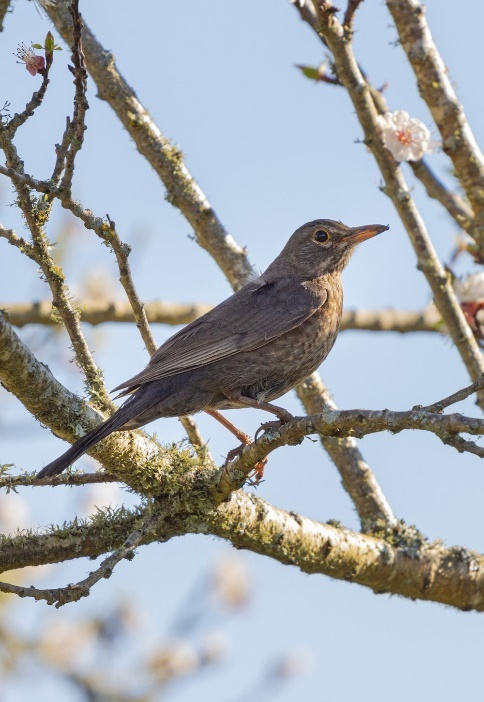
\includegraphics[width=.5\textwidth]{./imgs/img17.jpg}
\caption{Fonte: https://unsplash.com/pt-br/fotografias/Ux0bFtZJnKw. Acesso em 21/02/2023.}
\end{figure}

\begin{quote}
\textbf{Canção do exílio}

Minha terra tem palmeiras\\
Onde canta o Sabiá,\\
As aves, que aqui gorjeiam,\\
Não gorjeiam como lá.

Nosso céu tem mais estrelas,\\
Nossas várzeas têm mais flores,\\
Nossos bosques têm mais vida,\\
Nossa vida mais amores.

Em cismar, sozinho, à noite,\\
Mais prazer encontro eu lá;\\
Minha terra tem palmeiras,\\
Onde canta o Sabiá.

Minha terra tem primores,\\
Que tais não encontro eu cá;\\
Em cismar -- sozinho, à noite --\\
Mais prazer encontro eu lá;\\
Minha terra tem palmeiras,\\
Onde canta o Sabiá.

Não permita Deus que eu morra,\\
Sem que eu volte para lá;\\
Sem que desfrute os primores\\
Que não encontro por cá;\\
Sem qu'inda aviste as palmeiras,\\
Onde canta o Sabiá.

\fonte{DIAS, Gonçalves. \emph{Cantos.} Leipzig: F. A. Brockhaus, 1857.}
\end{quote}

Glossário:

Gorjear: cantar\\
Primor: perfeição\\
Qu'inda: que ainda

\begin{escolha}
\item Quantas estrofes o poema apresenta? Quantos versos há em cada
estrofe?

\linhas{2}
\coment{O poema apresenta cinco estrofes, sendo três estrofes com quatro versos
e duas estrofes com seis versos.}


\item Transcreva duas rimas do poema.

\linhas{2}
\coment{O aluno pode transcrever, por exemplo, a rima cá/sabiá e flores/amores.}


\item Que tipo de sentimento a primeira estrofe do poema expressa?

\linhas{2}
\coment{A primeira estrofe expressa um sentimento de tristeza, já que o poeta
fala da saudade que sente de sua terra.}
\end{escolha}


\colorsec{Treino}

\num{1} Leia o trecho do poema a seguir e responda à questão:

\begin{quote}
\textbf{Saudades}

Nas horas mortas da noite\\
Como é doce o meditar\\
Quando as estrelas cintilam\\
Nas ondas quietas do mar;\\
Quando a lua majestosa\\
Surgindo linda e formosa,\\
Como donzela vaidosa\\
Nas águas se vai mirar!

Nessas horas de silêncio,\\
De tristezas e de amor,\\
Eu gosto de ouvir ao longe,\\
Cheio de mágoa e de dor,\\
O sino do campanário\\
Que fala tão solitário\\
Com esse som mortuário\\
Que nos enche de pavor.

{[}...{]}.

\fonte{DE ABREU, Casimiro. Saudades. In: \emph{Cantos de tristeza e
de saudade}. Paris: Casa Editorial Franco-Ibero-Americana,
19-?.}
\end{quote}

Glossário

Campanário: torre\\
Cintilar: brilhar\\
Mirar: olhar

As estrofes reproduzidas acima apresentam

\begin{escolha}
\item oito versos.

\item dois versos.

\item versos sem rimas.

\item versos sem sentimentos.
\end{escolha}

\coment{Dificuldade: Fácil.

Saeb: Reconhecer diferentes modos de organização composicional de textos
em versos. BNCC: (EF35LP27) Ler e compreender, com certa autonomia,
textos em versos, explorando rimas, sons e jogos de palavras, imagens
poéticas (sentidos figurados) e recursos visuais e sonoros.

a) Correta. Cada estrofe apresenta oito versos (linhas);
b) Incorreta. O trecho acima apresenta duas estrofes, e não versos;
c) Incorreta. O poema apresenta rimas;
d) Incorreta. O gênero poesia se baseia na expressão de sentimentos.}

\num{2} Leia o trecho do poema a seguir e responda à questão:

\begin{quote}
\textbf{O Canto do Guerreiro}\\
\textbf{I}

Aqui na floresta\\
Dos ventos batida,\\
Façanhas de bravos\\
Não geram escravos,\\
Que estimem a vida\\
Sem guerra e lidar\\
--- Ouvi-me, Guerreiros,\\
--- Ouvi meu cantar.

{[}...{]}.

\fonte{DIAS, Gonçalves. O Canto do Guerreiro. In: \emph{Canto.}
Leipzig: F.A. Brockhaus, 1857.}
\end{quote}

Uma das rimas encontradas na estrofe acima é

\begin{escolha}
\item façanhas/não.

\item ouvi-me/ouvi.

\item lidar/cantar.

\item guerra/lidar.
\end{escolha}

\coment{Dificuldade: Média.

Saeb: Reconhecer diferentes modos de organização composicional de textos
em versos. BNCC: (EF35LP27) Ler e compreender, com certa autonomia,
textos em versos, explorando rimas, sons e jogos de palavras, imagens
poéticas (sentidos figurados) e recursos visuais e sonoros.

a) Incorreta. A sonoridade das palavras não é semelhante;
b) Incorreta. Embora os dois trechos apresentem palavras iguais, não é
estabelecida uma rima;
c) Correta. Os dois verbos são utilizados ao final de dois versos
diferentes, criando uma rima;
d) Incorreta. As duas palavras aparecem uma após a outra na estrofe.}

\num{3} Leia o trecho do poema a seguir e responda à questão:

\begin{quote}
\textbf{Sem Remédio}

{[}...{]}

E é desde então que eu sinto este pavor,\\
Este frio que anda em mim, e que gelou\\
O que de bom me deu Nosso Senhor!\\
Se eu nem sei por onde ando e onde vou!

{[}...{]}.

\fonte{ESPANCA, Florbela. Sem Remédio. In: \emph{Poemas
Selecionados.} São Paulo: Primavera Editorial, 2020.}
\end{quote}

A estrofe acima transmite um sentimento de

\begin{escolha}
\item alegria.

\item desespero.

\item aceitação.

\item entusiasmo.
\end{escolha}

\coment{Dificuldade: Difícil.

Saeb: Analisar a construção de sentidos de textos em versos com base em
seus elementos constitutivos. BNCC: (EF35LP31) Identificar, em textos
versificados, efeitos de sentido decorrentes do uso de recursos rítmicos
e sonoros e de metáforas.

a) Incorreta. A presença de termos negativos impede que o sentimento de
alegria seja identificado;
b) Correta. O uso de um termo como ``pavor'' expõe o sentimento de
desespero;
c) Incorreta. A poeta não aparenta aceitar os sentimentos negativos que
a acometem;
d) Incorreta. A poeta menciona ``Este frio que anda em mim {[}...{]}'',
demonstrando sofrimento.}

\chapter{6. Textos: modos variados de se escrever e falar}

\coment{Neste módulo, os alunos conhecerão o conceito de variedade linguística.
A ideia é compreender e diferenciar a língua culta das mais diferentes
formas de se comunicar, na fala e na escrita, considerando que apesar da
existência de normas, todas as manifestações lingüísticas podem ser
consideradas válidas, trabalhando a ideia de preconceito linguístico.\\
Habilidades BNCC: EF35LP22, EF35LP30}

\colorsec{Habilidades SAEB}

\begin{itemize}
\item Identificar as variedades linguísticas em textos.
\end{itemize}

\begin{figure}[htpb!]
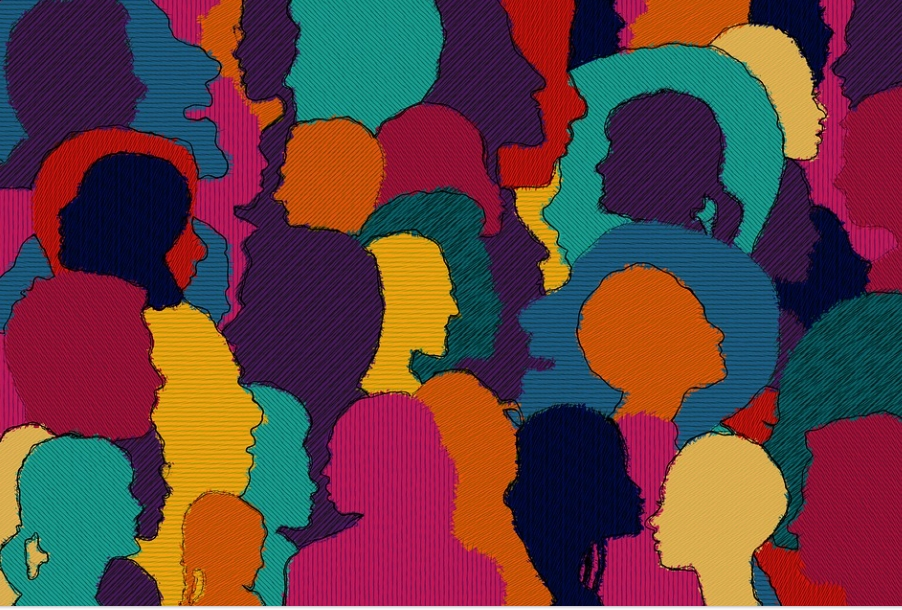
\includegraphics[width=.5\textwidth]{./imgs/img18.jpg}
\caption{Fonte: https://pixabay.com/pt/illustrations/diversidade-pessoas-cabe\%c3\%a7as-humanos-5582454/. Acesso 26/02/2023.}
\end{figure}

\conteudo{A Língua Portuguesa é muito diversa, assim como toda a cultura
brasileira. Nas mais diferentes regiões, é comum encontrarmos formas
diferentes de dizer as mesmas coisas. No Brasil, por exemplo, podemos
observar variações na pronúncia, no vocabulário e na gramática entre
diferentes regiões, como o sotaque carioca, o gaúcho, o nordestino,
entre outros. Além disso, diferentes grupos sociais, como os jovens ou
as pessoas mais velhas, podem ter maneiras diferentes de se expressar,
usando gírias, expressões próprias e formas de falar específicas.
Chamamos essas formas diferentes de falar de \textbf{variedades
linguísticas}. Todas elas fazem parte da riqueza e diversidade cultural
das diferentes comunidades que as falam e por isso devem ser respeitadas
e preservadas.

Lei ao texto a seguir, do romance \emph{Inocência}, do escritor Visconde
de Taunay. Observe, durante a sua leitura, os elementos de variedades
linguísticas.

\begin{quote}
Chegou-se o pai à cama e, com todo o carinho, chamou: Nocência!
Nocência! E como não a visse despertar logo, sacudiua com brandura até
que ela abrisse uns olhos espantados.

--- Apre! Que sono! disse o bondoso velho. Num instante que fui lá
dentro?!... Vamos, são horas de tomar a mezinha. {[}...{]}

--- Olhe, dona, aconselhou ele, beba de um só trago e chupe, logo
depois, uns gomos de limão-doce.

--- Então é muito mau? choramingou a doente.

--- É amargo; mas num gole mecê toma isto.

--- Papai, recalcitrou a moça, não quero... eu não quero.

--- Ora, filhinha do meu coração, não se canhe; é preciso... Amanhã há
de você sentir-se boa; não é doutor?

--- Com certeza, se tomar esta poção, assegurou Cirino.

---Depois, quando eu ir lá à vila, hei de trazer para você uma coisa
bonita... uns lavrados. Ouviu?

--- Nhor-sim.

--- Ande, Tico, acrescentou o mineiro voltando-se para o anão, vai
depressa buscar limão-doce; na cozinha há um meio cascado.
\end{quote}

\fonte{TAUNAY, Visconde de. \emph{Inocência}. Disponível:
http://objdigital.bn.br/Acervo\_Digital/livros\_eletronicos/inocencia.pdf.
Acesso em: 26 fev. 2023.}
}

\colorsec{Atividades}

\num{1} Após sua primeira leitura do texto, você acredita que a história
narrada se passa em uma época presente ou passada? Por quê?

\linhas{3}
\coment{Espera-se que os estudantes identifiquem o texto como se passando em uma
época passada a partir de marcas de variações linguísticas, como
``mecê'' e ``nhor-sim'', termos que não costumam mais ser utilizados
hoje.}


\num{2} Destaque alguns dos termos que você identificou, durante a sua
leitura, como variedades linguísticas.


\linhas{2}
\coment{Resposta pessoa. Sugestões: apre, mecê, canhe, Nhor-sim.}

\num{3} A partir de sua percepção sobre o contexto em que a história é
narrada, você diria que a cena se passa em uma área rural ou urbana? Por
quê?

\linhas{4}
\coment{A cena se passa em uma área rural, pois o pai faz referência a ir ``lá à
vila {[}...{]} trazer para você uma coisa bonita... uns lavrados''. Além
disso, podemos perceber pela linguagem dos personagens, como ``canhe'',
``cascado'', que se trata de um grupo sertanejo.}


\num{4} A palavra ``lavrados'' é um termo que no Brasil inteiro possui
vários significados bastante diferentes. Assinale as alternativas
verdadeiras (V) e falsas (F) que contêm a explicação do sentido correto
para a palavra, tendo em vista o contexto da cena:

\begin{boxlist}
\item Um campo ``lavrado'', isto é, plantado e cultivado. \coment{F}

\item Um documento ``lavrado'' em cartório, isto é, registrado e estabelecido. \coment{F}

\item Um tecido ``lavrado'', isto é, um tecido trabalhado e bordado para fazer vestido. \coment{V}

\item Um copo ``lavrado'', isto é, um copo de material barato usado em bares. \coment{F}
\end{boxlist}

\num{5} Observe novamente o texto. A jovem ``Nocência'' (apelido de
Inocência) utiliza um pronome de tratamento, para se referir ao pai, que
pode ser considerado um caso de variação linguística.

\begin{escolha}
\item Escreva-o na linha a seguir.

\linhas{1}
\coment{Nhor-sim.}

\item Qual é o seu significado?

\linhas{1}
\coment{O termo é equivalente a ``sim, senhor''.}
\end{escolha}

\num{6} Releia o trecho retirado do diálogo do romance.

\begin{quote}
--- Apre! Que sono! disse o bondoso velho. Num instante que fui lá
dentro?!... Vamos, são horas de tomar a mezinha.
\end{quote}

Considerando que nesse trecho ocorrem marcas de discurso direto, isto é,
o texto reproduz a fala do personagem. Identifique nessa fala uma
expressão utilizada por ele que pode ser considerado um caso de
variedade linguística.

\linhas{1}
\coment{A expressão: ``Apre!''.}


\num{7} Observe a foto a seguir e complete o espaço na frase com o termo
que nomeia o elemento mostrado. Como ele costuma ser nomeado em sua
região?

\begin{figure}[htpb!]
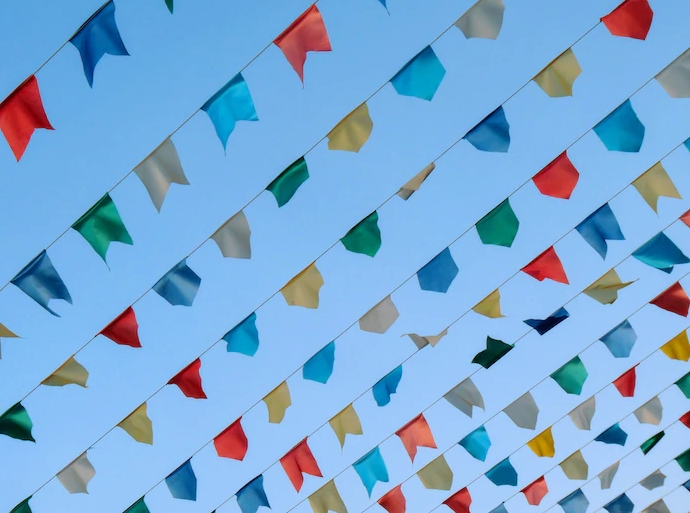
\includegraphics[width=.5\textwidth]{./imgs/img19.jpg}
\caption{Fonte: https://unsplash.com/pt-br/fotografias/UOAD9U-TYxc. Acesso em: 26/02/2023.}
\end{figure}

A \preencher de São João é uma decoração típica das
festas juninas no Brasil. São feitas de papel colorido e são penduradas
em fios ou cordas para decorar as ruas, praças e festas.

\coment{``Bandeirola'' na região Sudeste e ``bandeirinha'' na região Nordeste.}

\num{8} A mandioca é um alimento de origem indígena muito consumido em todo
o Brasil. Em outras regiões do Brasil ela possui outros nomes. Faça uma
pesquisa sobre os outros nomes, que representam variações linguísticas
do termo.

\linhas{1}
\coment{Macaxeira e Aipim.}


\num{9} Complete as lacunas com exemplos de variação lingüística para cada palavra:

\begin{escolha}
\item Ônibus \preencher. \coment{coletivo;}

\item Refrigerante \preencher. \coment{refri;}

\item Pão \preencher. \coment{pão de sal, cacetinho;}

\item Pipoca \preencher. \coment{poca, pipoquinha.}
\end{escolha}


\num{10} A partir do tema estudado, para você, qual é a importância de
aprender sobre as variedades linguísticas?

\linhas{4}

\coment{Resposta pessoal. É importante que os estudantes percebam que o
vocabulário se amplia com esse estudo de variedades linguísticas, além
de nos fazer ter uma percepção mais clara sobre as diferenças culturais
e sobre a importância do respeito a essas variedades, que são igualmente
válidas.}

\section{Treino}

\num{1} Leia o texto a seguir e responda à pergunta:

\begin{quote}
Cirino tomara a garrafa.

--- Isto, afirmou ele, acaba com certeza a cura.

E, esquivando-se de pronunciar o nome e a qualidade da pessoa de quem
estava tratando:

--- Ela há de ter hoje algum apetite e poderá levantar-se um pouco, pois
já tomou o seu caldinho.

--- Então, ao meio-dia, recomendou Pereira muito baixinho a Cirino,
vosmecê mande chamar a nossa doente e dê-lhe a \textbf{mezinha}. Ouviu?
Já avisei lá dentro...

\fonte{TAUNAY, Visconde de. \emph{Inocência}. Disponível:
http://objdigital.bn.br/Acervo\_Digital/livros\_eletronicos/inocencia.pdf.
Acesso em: 26 fev. 2023.}
\end{quote}

Selecione a alternativa que traz o significado correto da palavra em destaque ``mezinha'':

\begin{escolha}
\item Pequena mesa utilizada por médicos para o tratamento de doenças leves.

\item Remédio caseiro fabricado com ingredientes naturais, como ervas e frutas.

\item Espécie de vela utilizada em barcos grandes para regular as direções seguidas.

\item Andar intermediário localizado entre dois andares principais de um prédio.
\end{escolha}

\coment{Dificuldade: Média.

Saeb: Identificar as variedades linguísticas em textos.

a) Incorreta. O termo mais apropriado para o significado descrito seria
``mesinha'';
b) Correta. O termo ``mezinha'' refere-se a uma medicação natural;
c) Incorreta. O termo mais apropriado para o significado descrito seria
``mezanino'';
d) Incorreta. Incorreta. O termo mais apropriado para o significado
descrito seria ``mesinha''.}

\num{2} Leia o texto a seguir e responda à pergunta:

\begin{quote}
Levantou uns olhos súplices e, agarrando resolutamerte o remédio,
bebeu-o todo de um jacto. Depois deu um suspiro de enjôo e ficou com os
lábios entreabertos, à espera que o adocicado sumo do limão lhe tirasse
o amargor do medicamento.

--- Então, exclamou Pereira, era maior o medo que a coisa em si! Você
tomou a dose numa \textbf{relancina}.

\fonte{TAUNAY, Visconde de. \emph{Inocência}. Disponível:
http://objdigital.bn.br/Acervo\_Digital/livros\_eletronicos/inocencia.pdf.
Acesso em: 26 fev. 2023.}
\end{quote}

A palavra em destaque, ``relancina'' se trata de um regionalismo
utilizado no Rio Grande do Sul, podendo por isso ser chamado de
variedade lingüística. Selecione a alternativa que indica um sinônimo
para esse termo:

\begin{escolha}
\item rapidamente.

\item lentamente.

\item dificilmente.

\item pausadamente.
\end{escolha}

\coment{Dificuldade: Fácil.

Saeb: Identificar as variedades linguísticas em textos.

a) Correta. O termo ``relancina'' significa uma ação realizada
rapidamente;
b) Incorreta. O termo seria antônimo de ``relancina'';
c) Incorreta. Como ``relancina'' se refere a realizar algo rapidamente,
não há o sentido de dificuldade;
d) Incorreta. ``relancina'' tem o sentido de velocidade e prontidão,
então, não há sentido de pausa.}

\num{3} Leia o texto a seguir e responda à questão:

\begin{quote}
Ouvira Meyer estas indicações terapêuticas com os olhos muito fitos em
quem as dava: depois, voltando-se para Pereira, disse com um aprobatório
aceno de cabeça:

--- \emph{Pom} médico! \emph{pom} médico!

Desse momento em diante, votou Cirino ao alemão a mais decidida da
simpatia; e Pereira, presenciando o congraçamento daqueles dois homens,
de si pára si ilustres e incontestáveis sabichões, sentiu-se feliz por
abrigá-los a um tempo em sua humilde vivenda.

\fonte{TAUNAY, Visconde de. \emph{Inocência}. Disponível:
http://objdigital.bn.br/Acervo\_Digital/livros\_eletronicos/inocencia.pdf.
Acesso em: 26 fev. 2023.}
\end{quote}

O termo em destaque ``pom'' aparece como \textbf{discurso direto} do
personagem estrangeiro, representando um caso de variação linguística.
Assim, o termo indica:

\begin{escolha}
\item que o narrador escreve de maneira diferente da fala do personagem,
corrigindo sua fala.

\item que o personagem fala exatamente dessa forma, pois é discurso direto,
e assim mostra sua pronúncia.

\item que o narrador insere uma fala para a personagem mostrando um sentido
diferente e contrário.

\item que o trecho não reproduz exatamente a fala do personagem alemão,
pois é discurso direto.
\end{escolha}

\coment{Dificuldade: Difícil.

Saeb: Identificar as variedades linguísticas em textos.

Habilidades BNCC: EF35LP22, EF35LP30

a) Incorreta. Sendo discurso direto, o narrador reproduz exatamente a
fala do personagem;
b) Correta. Como é discurso direto, o personagem falou exatamente dessa
forma;
c) Incorreta. A definição de discurso direto se relaciona com a fala
exata da personagem, e não contrário;
d) Incorreta. Sendo discurso direto, sua definição pressupõe a fala
exata do personagem.}

\chapter{7. Palavras que acrescentam sentidos}

\coment{Os alunos serão apresentados às duas classes de palavras: adjetivos e
advérbios. Nesse momento, é importante compreender que essas palavras
acrescentam sentidos às outras, não tendo uma existência independente
nos textos lidos.}

\colorsec{Habilidades SAEB}

\begin{itemize}
\item Analisar os efeitos de sentido decorrentes do uso dos adjetivos.

\item Analisar os efeitos de sentido decorrentes do uso dos advérbios.
\end{itemize}

\begin{figure}[htpb!]
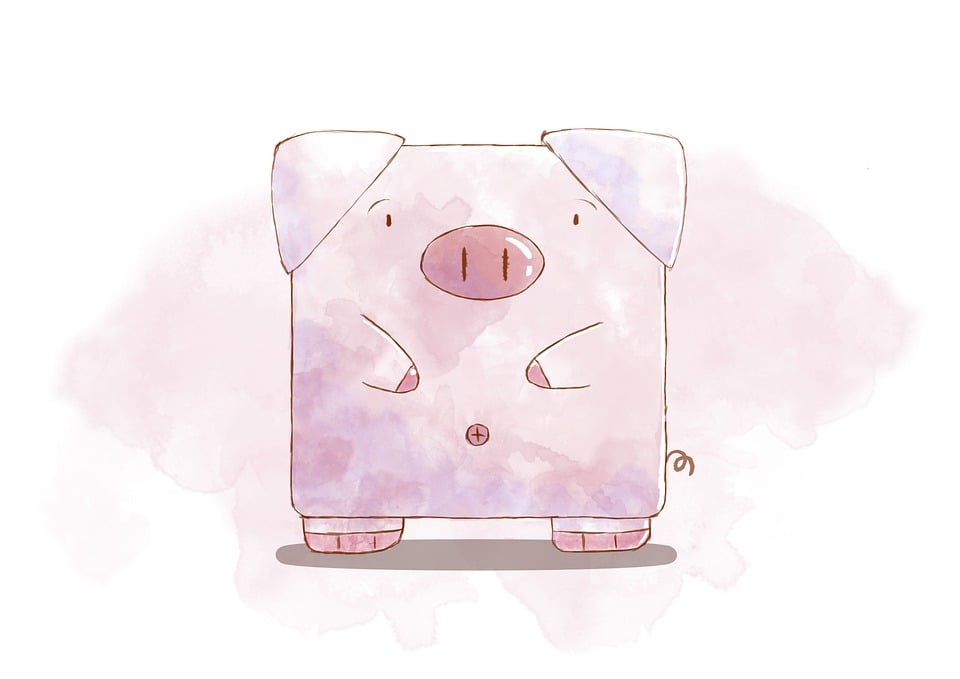
\includegraphics[width=.5\textwidth]{./imgs/img20.jpg}
\caption{Fonte: https://pixabay.com/pt/illustrations/porco-porco-de-desenho-animado-4417320/}
\end{figure}

\conteudo{Existem diversas maneiras de nos expressarmos textualmente. Quando
contamos uma história, é comum pensarmos em torná-la mais atraente e
descritiva. Uma forma importante de fazer isso é por meio de duas
classes de palavras: os adjetivos e os advérbios.

\begin{itemize}
\item
  Adjetivo qualifica ou caracteriza um substantivo, indicando
  características ou propriedades como cor, tamanho, forma, origem,
  estado, entre outras. Por exemplo: "O vestido azul", "o cachorro
  grande", "a casa antiga", "o menino feliz".
\item
  Advérbio modifica ou complementa o sentido de um verbo, um adjetivo ou
  outro advérbio, indicando circunstâncias como tempo, modo, lugar,
  intensidade, negação, afirmação, entre outras. Por exemplo: "Ela
  correu rapidamente", "ele cantou muito bem", "nós vamos sair agora",
  "eles nunca chegaram atrasados".
\end{itemize}

Vamos ler o conto a seguir, para compreendermos mais a função de
adjetivos e advérbios nas narrativas:

\textbf{Os três porquinhos}

Era uma vez três porquinhos aventureiros: o primeiro era preguiçoso e
gostava de dormir o dia todo, o segundo era vaidoso e passava horas se
admirando no espelho, e o terceiro era trabalhador e sempre ocupado
construindo sua casa com muito cuidado.

Um dia, um grande e malvado lobo apareceu na floresta, procurando uma
refeição saborosa para satisfazer sua fome voraz. O lobo farejou o ar e
logo sentiu o cheiro suculento dos porquinhos. Ele seguiu o cheiro até a
primeira casa, construída com palha e capim. O porquinho preguiçoso
dormia profundamente e nem sequer notou o lobo se aproximando. O lobo
soprou e soprou, até que a casa se desfez em pedaços, e o porquinho
preguiçoso fugiu correndo para a casa do segundo porquinho.

A casa do segundo porquinho era um pouco melhor, construída com madeira,
mas ainda assim era bastante frágil. O lobo chegou logo em seguida,
ansioso para devorar seu jantar. O lobo soprou e soprou, mas a casa
aguentou mais tempo do que a primeira. Porém, ainda assim não resistiu e
o porquinho vaidoso teve que fugir para a casa do terceiro porquinho.

A casa do terceiro porquinho era a mais forte de todas, feita de tijolos
sólidos e resistentes. Quando o lobo chegou, ele não conseguiu soprar a
casa e não conseguiu entrar pela porta, que estava trancada. O porquinho
trabalhador havia construído uma casa resistente e segura, protegendo a
si mesmo e seus irmãos dos perigos da floresta.

O lobo tentou enganar o porquinho esperto, mas ele não caiu em suas
mentiras e permaneceu firme em sua casa forte. O lobo, finalmente,
desistiu e foi embora para procurar outra refeição. Assim, os porquinhos
puderam viver seguros, sem medo dos perigos que espreitavam na floresta.

No conto, podemos notar como os adjetivos e advérbios são importantes em
uma historinha infantil. Eles tornam a narrativa mais rica em detalhes,
permitindo que o leitor se envolva e se identifique com os personagens e
as situações da história.}

\colorsec{Atividades}

\num{1} Qual é a personalidade de cada um dos três porquinhos?

\linhas{2}
\coment{Cada personagem é caracterizado por um adjetivo: o primeiro porquinho é
preguiçoso, o segundo é vaidoso e o terceiro é trabalhador.}


\num{2} Como essa caracterização por meio de adjetivos influencia a
história?

\linhas{3}
\coment{Essa caracterização influencia a história, pois é a personalidade de
cada um dos porquinhos que determina a qualidade da casa que eles
constroem e sua capacidade de resistir ao ataque do lobo.}


\num{3} De que maneira os adjetivos que explicam as personalidades dos
porquinhos auxiliam a narrativa a diferenciá-los entre si?

\linhas{4}
\coment{Os adjetivos utilizados ajudam a diferenciar suas personalidades e a
mostrar como cada um deles reage diante do perigo e da ameaça do lobo.
Enquanto o primeiro e o segundo porquinhos não dão muita importância à
construção de uma casa forte e resistente, o terceiro porquinho é
retratado como alguém responsável e cuidadoso.}


\num{4} Retome no texto a descrição das casas dos três porquinhos. Como as
três casas são descritas?

\linhas{2}
\coment{A primeira casa é descrita como sendo feita de palha e capim, a segunda
casa é feita de madeira e terceira casa é feita de tijolos.}


\num{5} De que maneira os adjetivos utilizados para descrever as três casas
contribuem para nos fazer entender o andamento da história?

\linhas{4}
\coment{A primeira casa de palha é entendida como frágil, podendo ser atacada
pelo lobo. A segunda é entendida como mais resistente, mas não o
suficiente para suportar o sopro do lobo. Já a casa de tijolos é sólida
e resistente, o que a torna a mais forte de todas e capaz de resistir ao
ataque do lobo.}


\num{6} Como as descrições das casas contribuem para a criação de um
ambiente e de uma atmosfera específicos na narrativa?

\linhas{5}
\coment{A primeira casa de palha transmite uma sensação de fragilidade, criando
um ambiente de perigo e de ameaça. A segunda casa de madeira transmite
uma sensação de resistência e de esperança, mas ainda assim há a
sensação de perigo. Já a descrição da terceira casa como sendo feita de
tijolos sólidos e resistentes transmite uma sensação de proteção,
criando um ambiente de tranquilidade e segurança.}

\num{7} Cite advérbios usados no conto "Os Três Porquinhos".

\linhas{2}
\coment{Exemplos de advérbios utilizados no conto são: ``profundamente'',
``logo'', ``em seguida'', ``mais'', ``bastante'', ``firmemente'' e
``finalmente''.}

\num{8} Relacione as colunas entre os advérbios e as funções que eles
exercem ao longo do conto:

\begin{multicols}{2}
(1) Profundamente\medskip

(2) Logo\medskip

(3) Bastante\medskip

(4) Mais

\columnbreak

(\coment{3}) Quantidade

(\coment{2}) Tempo

(\coment{4}) Intensidade

(\coment{1}) Intensidade
\end{multicols}

\num{9} Na oração ``O lobo soprou e soprou, até que a casa se desfez em
pedaços", qual é a função do advérbio ``até''?

\linhas{3}
\coment{O advérbio "até" é usado para descrever a continuidade da ação, que se
interrompe em um certo limite, indicando que o lobo soprou repetidamente
até que a casa se quebrou completamente.}


\num{10} Retome o conto. Qual é o sentido do advérbio ``profundamente''?

\linhas{4}
\coment{O advérbio "profundamente" descreve como o porquinho preguiçoso estava
dormindo quando o lobo chegou: "O porquinho preguiçoso dormia
profundamente e nem sequer notou o lobo se aproximando." Esse advérbio
ajuda a dar ênfase na preguiça do porquinho, além de indicar que ele
estava dormindo de maneira muito intensa.}


\chapter{8. Fatos e opiniões}

\coment{Neste módulo, os alunos vão entrar em contato com as diferenças entre
fatos e opiniões. É importante estabelecer essa diferenciação, pois ela
permite reconhecer \emph{fake news} e ainda suscita um diálogo saudável
e mais produtivo em sala de aula e na vida em sociedade.\\
Habilidades BNCC: EF05LP16.}

\colorsec{Habilidades SAEB}

\begin{itemize}
\item Distinguir fatos de opiniões em textos.

\item Avaliar a fidedignidade de informações sobre um mesmo fato veiculadas
em diferentes mídias.
\end{itemize}

\begin{figure}[htpb!]
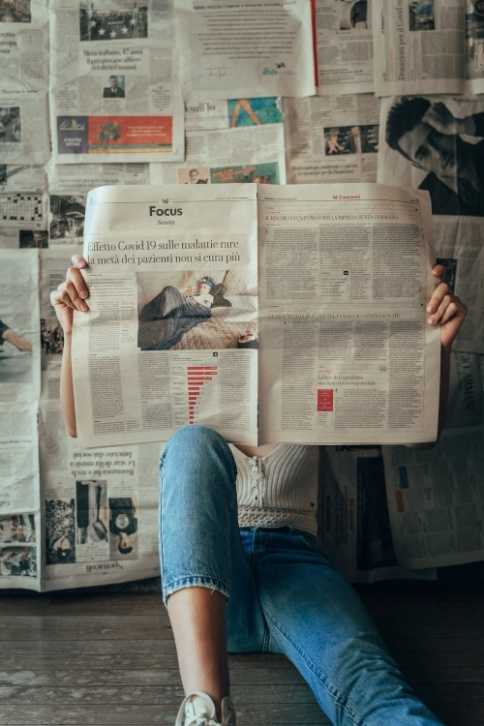
\includegraphics[width=.5\textwidth]{./imgs/img21.jpg}
\caption{Fonte: https://unsplash.com/pt-br/fotografias/Bc\_y35IwUHw. Acesso 20/02/2023.}
\end{figure}

\conteudo{Em nossa comunicação cotidiana, é muito comum que nos deparemos com
fatos e opiniões. Você sabe qual é a diferença entre eles?

Fatos são informações objetivas que podem ser comprovadas por evidências
ou dados verificáveis. Assim, eles são baseados em observações e
medidas, e não dependem de crenças pessoais ou pontos de vista. Podemos
considerar exemplos de fatos a temperatura de um local, o número de
habitantes de uma cidade ou o resultado de uma eleição.

Por outro lado, as opiniões são refletem nossos pensamentos, crenças ou
sentimentos pessoais. Assim, são subjetivas e podem variar de pessoa
para pessoa, pois cada um tem a sua própria experiência de vida e seus
valores, emoções e até mesmo preconceitos. Por esse motivo, podemos
achar uma comida gostosa enquanto nosso amigo acha ruim, ou ele pode
gostar de um filme, uma roupa, uma cor etc. e nós não.}

Leia o texto a seguir.

\begin{quote}
\textbf{Vacina contra Covid-19: notícia errada vira link mais
compartilhado pelo Facebook nos EUA}

O Facebook divulgou um relatório com os links mais vistos na rede social
nos Estados Unidos no primeiro trimestre de 2021, e em primeiro lugar
aparece uma notícia no site de um jornal americano que atribuiu
equivocadamente a morte de um médico à vacina contra a Covid-19.

Depois, o conteúdo da matéria foi atualizado para informar que uma
análise de peritos apontou não haver evidências de que a vacinação
causou a morte do homem duas semanas depois --- mas a esta altura, o
texto já havia se tornado muito popular entre movimentos negacionistas
contra as vacinas.

No total, o link teve 54 milhões de visualizações de usuários do
Facebook, segundo o relatório Widely Viewed Content.

O Centro de Controle de Doenças (CDC) do Departamento de Saúde dos EUA
afirma que milhares de ensaios clínicos já realizados no mundo, além de
pesquisas com dados populacionais, mostram que as vacinas contra a
Covid-19 são seguras e eficazes.

{[}...{]} Repórter da BBC especializada em redes sociais e
desinformação, Marianna Spring explica que a ampla disseminação do link
tem a ver com a atuação de "uma rede comprometida de ativistas"
antivacina, que encontram no Facebook um ambiente fértil para
distribuição desse tipo de conteúdo.

"Promover histórias emotivas e pessoais como esta (do médico) no
Facebook tem sido uma das principais táticas destes grupos para barrar
as pessoas de serem vacinadas --- mesmo quando, como aconteceu neste
caso, não há nenhuma evidência de ligação entre a vacina contra a
covid-19 e a morte", explica Spring.

\fonte{Link: https://www.bbc.com/portuguese/internacional-58312501}
\end{quote}

É muito importante distinguir fatos de opiniões porque quando as pessoas
as confundem, elas podem transmitir informações imprecisas ou mesmo
falsas, o que pode levar a mal-entendidos ou decisões equivocadas. Além
disso, isso garante um debate saudável e uma sociedade mais informada.

\colorsec{Atividades}

\num{1} Qual foi a notícia mais compartilhada no Facebook nos Estados
Unidos no primeiro trimestre de 2021?

\linhas{2}
\coment{Uma notícia no site de um jornal americano que atribuiu equivocadamente
a morte de um médico à vacina contra a Covid-19.}


\num{2} Por que essa notícia foi considerada equivocada?

\linhas{2}
\coment{Porque a análise de peritos apontou não haver evidências de que a
vacinação causou a morte do homem.}


\num{3} Qual foi a correção feita na matéria?

\linhas{2}
\coment{A matéria foi atualizada para informar que não havia evidências de que a
vacinação causou a morte do médico.}


\num{4} Por que o link se tornou popular entre movimentos negacionistas
contra as vacinas?

\linhas{3}
\coment{Porque encontram no Facebook um ambiente fértil para distribuição desse
tipo de conteúdo e porque promovem histórias emotivas e pessoais para
barrar as pessoas de serem vacinadas.}


\num{5} Quantas visualizações o link teve no total?

\linhas{2}
\coment{54 milhões de visualizações de usuários do Facebook, segundo o relatório
Widely Viewed Content.}


\num{6} O que o Centro de Controle de Doenças afirma sobre as vacinas
contra a Covid-19?

\linhas{2}
\coment{Afirma que milhares de ensaios clínicos já realizados no mundo, além de
pesquisas com dados populacionais, mostram que as vacinas contra a
Covid-19 são seguras e eficazes.}


\num{7} Por que a ampla disseminação do link no Facebook tem a ver com uma
rede de ativistas antivacina?

\linhas{2}
\coment{Porque esses ativistas encontram no Facebook um ambiente fértil para
distribuição desse tipo de conteúdo.}


\num{8} Qual tem sido uma das principais táticas desses grupos para barrar
as pessoas de serem vacinadas, de acordo com Marianna Spring?

\linhas{2}
\coment{Promover histórias emotivas e pessoais como a do médico atribuída
equivocadamente à vacina contra a Covid-19 no Facebook.}


\num{9} Podemos entender, de acordo com o texto, que as notícias falsas são
propagadas por fatos ou por opiniões? Justifique sua resposta.

\linhas{2}
\coment{As notícias falsas são propagadas por opiniões, pois são baseadas em
histórias emotivas e emocionais, e não baseadas em dados objetivos da
realidade.}


\num{10} Em sua opinião, de que maneira a disseminação de notícias falsas
impacta a busca por medidas de saúde mais eficazes?

\linhas{3}
\coment{Resposta pessoal. Espera-se que os alunos compreendam que as notícias
falsas podem gerar grandes malefícios, danos e até mesmo a morte de
muitas pessoas, nos casos de se voltarem aos temas de saúde e ciências.}

\colorsec{Treino}

\num{1} Leia o texto a seguir e responda à pergunta:

\begin{quote}
\textbf{Vacina contra Covid-19: notícia errada vira link mais
compartilhado pelo Facebook nos EUA}

O Facebook divulgou um relatório com os links mais vistos na rede social
nos Estados Unidos no primeiro trimestre de 2021, e em primeiro lugar
aparece uma notícia no site de um jornal americano que atribuiu
equivocadamente a morte de um médico à vacina contra a Covid-19.

Depois, o conteúdo da matéria foi atualizado para informar que uma
análise de peritos apontou não haver evidências de que a vacinação
causou a morte do homem duas semanas depois --- mas a esta altura, o
texto já havia se tornado muito popular entre movimentos negacionistas
contra as vacinas.

No total, o link teve 54 milhões de visualizações de usuários do
Facebook, segundo o relatório Widely Viewed Content.

O Centro de Controle de Doenças (CDC) do Departamento de Saúde dos EUA
afirma que milhares de ensaios clínicos já realizados no mundo, além de
pesquisas com dados populacionais, mostram que as vacinas contra a
Covid-19 são seguras e eficazes.

{[}...{]} Repórter da BBC especializada em redes sociais e
desinformação, Marianna Spring explica que a ampla disseminação do link
tem a ver com a atuação de "uma rede comprometida de ativistas"
antivacina, que encontram no Facebook um ambiente fértil para
distribuição desse tipo de conteúdo.

"Promover histórias emotivas e pessoais como esta (do médico) no
Facebook tem sido uma das principais táticas destes grupos para barrar
as pessoas de serem vacinadas --- mesmo quando, como aconteceu neste
caso, não há nenhuma evidência de ligação entre a vacina contra a
covid-19 e a morte", explica Spring.

\fonte{Link:
https://www.bbc.com/portuguese/internacional-58312501}
\end{quote}

Qual é a explicação da repórter Marianna Spring para a ampla
disseminação da notícia errada sobre a vacina contra a Covid-19 no
Facebook?

\begin{escolha}
\item A notícia falsa foi patrocinada por grandes empresas farmacêuticas,
que querem controlar a narrativa em torno das vacinas.

\item A notícia falsa foi compartilhada por engano por usuários inocentes
do Facebook.

\item A notícia falsa foi compartilhada por uma rede comprometida de
ativistas antivacina, que encontram no Facebook um ambiente fértil para
distribuição de conteúdo desinformativo.

\item A notícia falsa foi divulgada por políticos que se opõem às vacinas
contra a Covid-19.
\end{escolha}

\coment{Dificuldade: Difícil.

Saeb: Distinguir fatos de opiniões em textos. Avaliar a fidedignidade de
informações sobre um mesmo fato veiculadas em diferentes mídias. BNCC:
EF05LP16.

a) Incorreta. Essa afirmação não é sustentada pelo texto, pois não há
nenhuma menção às empresas farmacêuticas no texto;
b) Incorreta. A disseminação da notícia errada sobre a vacina contra a
Covid-19 se deve principalmente à rede antivacina que usa táticas
específicas para promover conteúdo desinformativo;
c) Correta. A notícia falsa foi compartilhada por uma rede de ativistas
antivacina, ou seja, foi algo intencional;
d) Incorreta. Não há nenhuma menção a políticos que se opõem às vacinas
contra a Covid-19 no texto.}

\num{2} Leia o texto a seguir e responda à pergunta:

\begin{quote}
\textbf{Vacina contra Covid-19: notícia errada vira link mais
compartilhado pelo Facebook nos EUA}

O Facebook divulgou um relatório com os links mais vistos na rede social
nos Estados Unidos no primeiro trimestre de 2021, e em primeiro lugar
aparece uma notícia no site de um jornal americano que atribuiu
equivocadamente a morte de um médico à vacina contra a Covid-19.

Depois, o conteúdo da matéria foi atualizado para informar que uma
análise de peritos apontou não haver evidências de que a vacinação
causou a morte do homem duas semanas depois --- mas a esta altura, o
texto já havia se tornado muito popular entre movimentos negacionistas
contra as vacinas.

No total, o link teve 54 milhões de visualizações de usuários do
Facebook, segundo o relatório Widely Viewed Content.

O Centro de Controle de Doenças (CDC) do Departamento de Saúde dos EUA
afirma que milhares de ensaios clínicos já realizados no mundo, além de
pesquisas com dados populacionais, mostram que as vacinas contra a
Covid-19 são seguras e eficazes.

{[}...{]} Repórter da BBC especializada em redes sociais e
desinformação, Marianna Spring explica que a ampla disseminação do link
tem a ver com a atuação de "uma rede comprometida de ativistas"
antivacina, que encontram no Facebook um ambiente fértil para
distribuição desse tipo de conteúdo.

"Promover histórias emotivas e pessoais como esta (do médico) no
Facebook tem sido uma das principais táticas destes grupos para barrar
as pessoas de serem vacinadas --- mesmo quando, como aconteceu neste
caso, não há nenhuma evidência de ligação entre a vacina contra a
covid-19 e a morte", explica Spring.

\fonte{Link:
https://www.bbc.com/portuguese/internacional-58312501}
\end{quote}

Qual é o objetivo principal do artigo sobre a notícia errada da vacina
contra a Covid-19?

\begin{escolha}
\item Mostrar que a vacinação contra a Covid-19 pode causar morte.

\item Explicar como o Facebook pode ser usado para espalhar desinformação sobre vacinas.

\item Argumentar que as pessoas não devem confiar nas vacinas contra a Covid-19.

\item Defender que a notícia errada foi compartilhada por ativistas pró-vacinação.
\end{escolha}

\coment{Dificuldade: Fácil

Saeb: Distinguir fatos de opiniões em textos. Avaliar a fidedignidade de
informações sobre um mesmo fato veiculadas em diferentes mídias. BNCC:
EF05LP16.

a) Incorreta. As vacinas são descritas como sendo seguras, por terem
sido desenvolvidas segundo normas científicas;
b) Correta. O artigo se concentra em explicar como uma notícia errada
foi compartilhada no Facebook e se tornou viral devido a uma rede
comprometida de ativistas antivacina;
c) Incorreta. O texto mostra que as informações sobre a insegurança das
vacinas são falsas, e portanto as pessoas podem confiar na ciência;
d) Incorreta. O texto mostra que, pelo contrário, foram os ativistas
anti-vacina que divulgaram notícias falsas.}

\num{3} Leia o texto a seguir e responda à pergunta:

\begin{quote}
\textbf{Vacina contra Covid-19: notícia errada vira link mais
compartilhado pelo Facebook nos EUA}

O Facebook divulgou um relatório com os links mais vistos na rede social
nos Estados Unidos no primeiro trimestre de 2021, e em primeiro lugar
aparece uma notícia no site de um jornal americano que atribuiu
equivocadamente a morte de um médico à vacina contra a Covid-19.

Depois, o conteúdo da matéria foi atualizado para informar que uma
análise de peritos apontou não haver evidências de que a vacinação
causou a morte do homem duas semanas depois --- mas a esta altura, o
texto já havia se tornado muito popular entre movimentos negacionistas
contra as vacinas.

No total, o link teve 54 milhões de visualizações de usuários do
Facebook, segundo o relatório Widely Viewed Content.

O Centro de Controle de Doenças (CDC) do Departamento de Saúde dos EUA
afirma que milhares de ensaios clínicos já realizados no mundo, além de
pesquisas com dados populacionais, mostram que as vacinas contra a
Covid-19 são seguras e eficazes.

{[}...{]} Repórter da BBC especializada em redes sociais e
desinformação, Marianna Spring explica que a ampla disseminação do link
tem a ver com a atuação de "uma rede comprometida de ativistas"
antivacina, que encontram no Facebook um ambiente fértil para
distribuição desse tipo de conteúdo.

"Promover histórias emotivas e pessoais como esta (do médico) no
Facebook tem sido uma das principais táticas destes grupos para barrar
as pessoas de serem vacinadas --- mesmo quando, como aconteceu neste
caso, não há nenhuma evidência de ligação entre a vacina contra a
covid-19 e a morte", explica Spring.

\fonte{Link:
https://www.bbc.com/portuguese/internacional-58312501}
\end{quote}

Qual é o objetivo do CDC em relação às vacinas contra a Covid-19?

\begin{escolha}
\item Desencorajar as pessoas a tomarem as vacinas.

\item Estimular a ampla disseminação de notícias falsas sobre as vacinas.

\item Defender a segurança e eficácia das vacinas contra a Covid-19.

\item Ignorar as pesquisas com dados populacionais sobre as vacinas.
\end{escolha}

\coment{Dificuldade: Média.

Saeb: Distinguir fatos de opiniões em textos. Avaliar a fidedignidade de
informações sobre um mesmo fato veiculadas em diferentes mídias. BNCC:
EF05LP16.

a) Incorreta. O CDC defende a eficácia das vacinas, por isso incentiva
que as pessoas as tomem;
b) Incorreta. O CDC busca divulgar notícias baseadas em fatos para
evitar a disseminção de notícias falsas;
c) Correto. O CDC busca encorajar o conhecimento e a propagação das
vacinas, já que são comprovadamente eficazes;
d) Incorreta. O CDC baseia-se em pesquisas científicas organizadas em
dados para defender as vacinas, dentre elas os dados populacionais.}

\chapter{9. Organizando dados}

\coment{Os alunos serão apresentados a dois modos bastante comuns de organizar
dados: os gráficos e as tabelas. É importante que compreendam como ambos
se organizam e as facilidades que eles trazem para a organização e
compreensão de dados, pois são formas de organizar dados de maneira
visualmente facilitada.\\
Habilidades BNCC: EF05LP23.}

\colorsec{Habilidades SAEB}

\begin{itemize}
\item Analisar informações apresentadas em gráficos, infográficos ou tabelas.
\end{itemize}

\begin{figure}[htpb!]
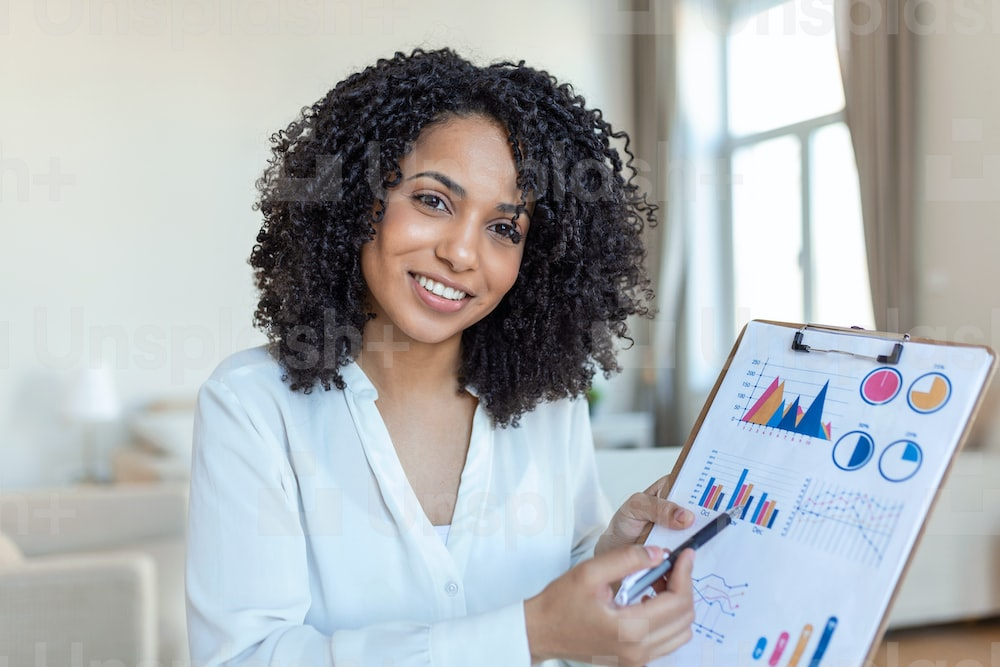
\includegraphics[width=.5\textwidth]{./imgs/img22.jpg}
\caption{Fonte: https://unsplash.com/pt-br/fotografias/Jy2mwPtOCOU}
\end{figure}

\conteudo{Você já ouviu falar em gráficos? Sabe para que servem? Os gráficos são
ferramentas muito úteis para nos ajudar a entender informações
importantes. Eles são como desenhos que mostram dados de uma forma fácil
de entender.

Por exemplo, se quisermos saber quantas pessoas gostam de chocolate e
quantas pessoas preferem baunilha, podemos fazer uma pesquisa e colocar
os resultados em um gráfico. Assim, a pizza inteira representa a
totalidade de pessoas pesquisadas, a ``fatia'' azul a quantidade de
pessoas que prefere o sabor de chocolate e a ``fatia'' vermelha a
quantidade que prefere baunilha. Nele podemos ver claramente quantas
pessoas escolheram cada sabor:

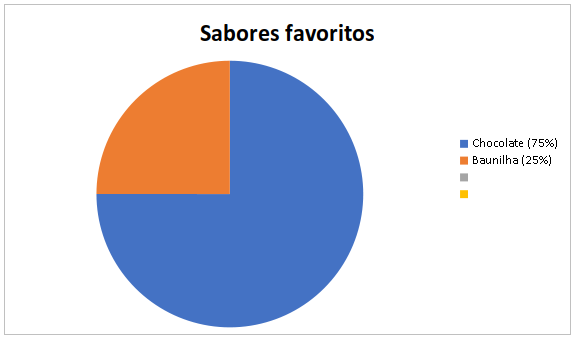
\includegraphics[width=.5\textwidth]{./imgs/chart1.png}

Os gráficos são parecidos com desenhos, e nos ajudam a ver como os dados
estão distribuídos. Por exemplo, se quisermos saber a quantidade de
frutas que foram vendidas em uma loja durante um mês, podemos fazer um
gráfico de barras. Cada barra representa a quantidade de uma fruta
vendida, e podemos comparar facilmente as quantidades. No gráfico de
barras, as quantidades são representadas visualmente por barras que
crescem conforme o número cresce. Assim, no gráfico a seguir podemos
observar que as bananas foram as frutas mais vendidas na quitanda
durante o mês.

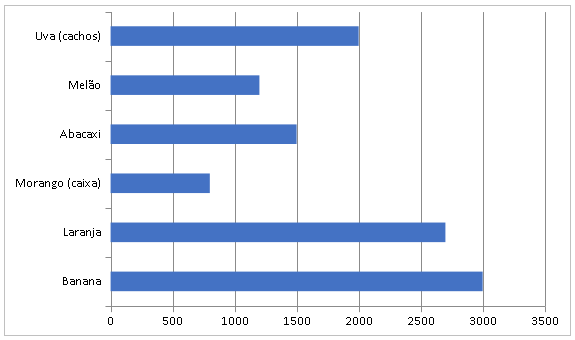
\includegraphics[width=.5\textwidth]{./imgs/chart2.png}

Os gráficos e tabelas são muito importantes em muitas áreas, como na
ciência, na economia e até mesmo no esporte. Eles ajudam a nos comunicar
informações importantes de forma clara e fácil de entender.}

\colorsec{Atividades}

\num{1} O que é um gráfico de barra?

\linhas{1}
\coment{Um gráfico que mostra quantidades diferentes de algo usando barras
verticais.}


\num{2} Para que serve um gráfico de barra?

\linhas{1}
\coment{Serve para comparar quantidades de coisas diferentes.}


\num{3} O que é um gráfico de pizza?

\linhas{1}
\coment{Um gráfico que mostra porcentagens de algo usando pedaços de uma torta.}

\num{4} Para que serve um gráfico de pizza?

\linhas{1}
\coment{Serve para mostrar a proporção de algo em relação ao todo.}


\num{5} Como podemos comparar quantidades usando um gráfico de barra?

\linhas{1}
\coment{Comparando a altura das barras verticais.}

\num{6} Observe o seguinte gráfico.

\begin{figure}[htpb!]
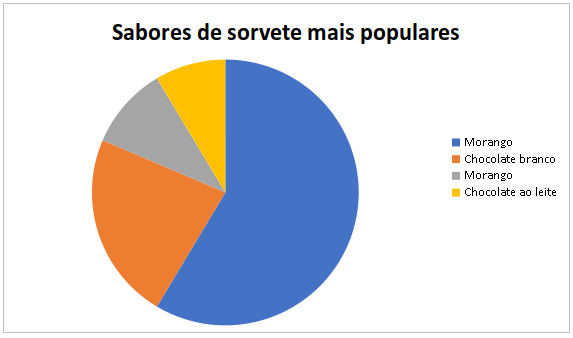
\includegraphics[width=.5\textwidth]{./imgs/chart3.png}
\end{figure}

\begin{escolha}
\item Como podemos saber qual é o sabor de sorvete mais popular usando um
gráfico de pizza?

\linhas{1}
\coment{Olhando para o tamanho do pedaço correspondente ao sabor de sorvete.}


\item Qual sabor de sorvete é mais popular, segundo o gráfico?

\linhas{1}
\coment{O sorvete de morango.}
\end{escolha}


\num{7} Qual é a diferença entre um gráfico de barra e um gráfico de pizza?

\linhas{2}
\coment{Um gráfico de barra usa barras verticais e um gráfico de pizza usa
pedaços de uma torta para mostrar informações.}


\num{8} Qual é a semelhança entre um gráfico de barra e um gráfico de
pizza?

\linhas{1}
\coment{Ambos são usados para representar informações de uma forma visual.}


\num{9} Selecione as alternativas verdadeiras (V) ou falsas (F): quais são
as informações que podemos representar usando um gráfico de barra?

\begin{boxlist}
\item Livros \coment{V}

\item Tristeza \coment{F}

\item Beleza \coment{F}

\item Sabores \coment{V}

\item Legumes \coment{V}
\end{boxlist}

\num{10} Quais são as informações que podemos representar usando um gráfico
de pizza?

\linhas{2}
\coment{Porcentagens e proporções de um todo, como a distribuição de um grupo em
relação a uma característica específica.}

\colorsec{Treino}

\num{1} Leia o texto a seguir e responda à questão:

\begin{quote}
Em 12 de maio, o Brasil registrou 9,3 mil novos casos de covid-19,
totalizando 177 mil notificações e 12,4 mil mortes. Mas o que esses e
outros dados significam e revelam sobre a realidade da doença no Brasil?
{[}...{]}

Atualmente {[}maio de 2020{]}, quase não há mais leitos de UTI no
sistema público de saúde de parte dos Estados, os casos e as mortes
estão aumentando --- mas a uma velocidade que tem caído ou se mantido
constante ---, há cada vez mais cidades pequenas atingidas e as pessoas
têm respeitado menos o distanciamento social.

{[}...{]}

Mas também dá para entender a situação a partir de dados divulgados
pelos Estados sobre a ocupação de leitos UTI da rede pública.

Em 10 de maio, no Piauí, a taxa de ocupação dos leitos UTI para covid-19
era de 43\%. No Espírito Santo, 63\%. Em São Paulo, 69\%. No Ceará, em
Roraima, no Maranhão, em Pernambuco e no Rio de Janeiro, passa de 90\%.

\begin{figure}[htpb!]
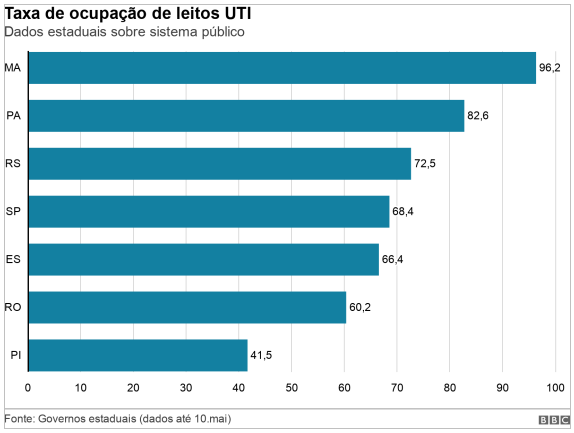
\includegraphics[width=.5\textwidth]{./imgs/img23.png}
\end{figure}

\fonte{Link: https://www.bbc.com/portuguese/brasil-52595760}
\end{quote}

Qual é a taxa de ocupação dos leitos UTI para covid-19 no estado de São
Paulo em 10 de maio de 2020, de acordo com os dados divulgados no texto?

\begin{escolha}
\item 43\%

\item 63\%

\item 69\%

\item Mais de 90\%
\end{escolha}

\coment{Dificuldade: Fácil.

Habilidades SAEB: Analisar informações apresentadas em gráficos,
infográficos ou tabelas. Habilidades BNCC: EF05LP23.

a) Incorreto. A taxa se refere ao estado do Piauí;
b) Incorreto. A taxa se refere ao estado do Espírito Santo;
c) Correto. A taxa se refere ao estado de São Paulo;
d) Incorreto. A taxa se refere aos estados de Pernambuco e Rio de
Janeiro.}

\num{2} Leia o texto a seguir e responda à questão:

\begin{quote}
Em 12 de maio, o Brasil registrou 9,3 mil novos casos de covid-19,
totalizando 177 mil notificações e 12,4 mil mortes. Mas o que esses e
outros dados significam e revelam sobre a realidade da doença no Brasil?
{[}...{]}

Atualmente {[}maio de 2020{]}, quase não há mais leitos de UTI no
sistema público de saúde de parte dos Estados, os casos e as mortes
estão aumentando --- mas a uma velocidade que tem caído ou se mantido
constante ---, há cada vez mais cidades pequenas atingidas e as pessoas
têm respeitado menos o distanciamento social.

{[}...{]}

Mas também dá para entender a situação a partir de dados divulgados
pelos Estados sobre a ocupação de leitos UTI da rede pública.

Em 10 de maio, no Piauí, a taxa de ocupação dos leitos UTI para covid-19
era de 43\%. No Espírito Santo, 63\%. Em São Paulo, 69\%. No Ceará, em
Roraima, no Maranhão, em Pernambuco e no Rio de Janeiro, passa de 90\%.

\begin{figure}[htpb!]
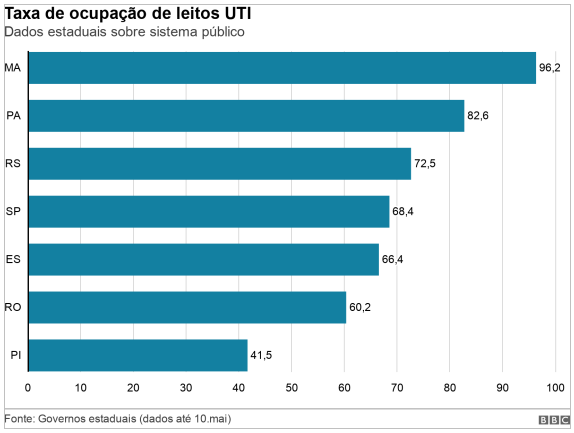
\includegraphics[width=.5\textwidth]{./imgs/img23.png}
\end{figure}
\fonte{Link:
https://www.bbc.com/portuguese/brasil-52595760}
\end{quote}

Quantos novos casos de covid-19 o Brasil registrou em 12 de maio de 2020, de acordo com o texto?

\begin{escolha}
\item 177 mil

\item 12,4 mil

\item 9,3 mil

\item Não há informação suficiente no texto para responder.
\end{escolha}

\coment{Dificuldade: Média.

Habilidades SAEB: Analisar informações apresentadas em gráficos,
infográficos ou tabelas. Habilidades BNCC: EF05LP23.

a) Incorreto. A taxa se refere às notificações de Covid no Brasil;
b) Incorreto. A taxa se refere ao número de mortes no país;
c) Correto. A taxa se refere aos novos casos de Covid;
d) Incorreto. O texto fornece dados suficientes para a resposta.}

\num{3} Leia o texto a seguir e responda à questão:

\begin{quote}
Em 12 de maio, o Brasil registrou 9,3 mil novos casos de covid-19,
totalizando 177 mil notificações e 12,4 mil mortes. Mas o que esses e
outros dados significam e revelam sobre a realidade da doença no Brasil?
{[}...{]}

Atualmente {[}maio de 2020{]}, quase não há mais leitos de UTI no
sistema público de saúde de parte dos Estados, os casos e as mortes
estão aumentando --- mas a uma velocidade que tem caído ou se mantido
constante ---, há cada vez mais cidades pequenas atingidas e as pessoas
têm respeitado menos o distanciamento social.

{[}...{]}

Mas também dá para entender a situação a partir de dados divulgados
pelos Estados sobre a ocupação de leitos UTI da rede pública.

Em 10 de maio, no Piauí, a taxa de ocupação dos leitos UTI para covid-19
era de 43\%. No Espírito Santo, 63\%. Em São Paulo, 69\%. No Ceará, em
Roraima, no Maranhão, em Pernambuco e no Rio de Janeiro, passa de 90\%.

\begin{figure}[htpb!]
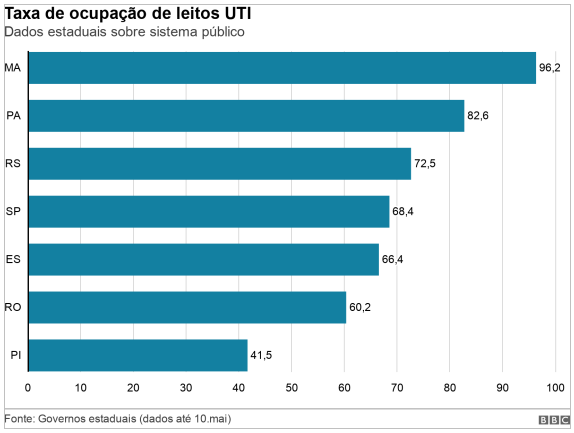
\includegraphics[width=.5\textwidth]{./imgs/img23.png}
\end{figure}
\fonte{Link: https://www.bbc.com/portuguese/brasil-52595760}
\end{quote}

A partir da leitura do gráfico, qual foi o estado brasileiro que teve
maior taxa de ocupação de leitos na UTI?

\begin{escolha}
\item PA (Pará)

\item RO (Roraima)

\item SP (São Paulo)

\item MA (Maranhão)
\end{escolha}

\coment{Dificuldade: Difícil.

Habilidades SAEB: Analisar informações apresentadas em gráficos,
infográficos ou tabelas. Habilidades BNCC: EF05LP23.

a) Incorreto. O Pará teve taxa de 82,6, menor que a do Maranhão, com
96,2;
b) Incorreto. Roraima teve taxa de 60,2, menor que a do Maranhão, com
96,2;
c) Incorreto. São Paulo teve taxa de 68,4, menor que a do Maranhão, com
96,2;
d) Correto. A taxa do Maranhão (maior faixa do gráfico) foi de 96,2.}

\chapter{10. Passo a passo}

\coment{Os alunos serão apresentados ao tema da progressão textual, entendendo
que os textos são organizados em sequencias, organizados tendo por base
nosso conhecimento de mundo e novas informações introduzidas pelo
próprio texto.\\
Habilidades BNCC: EF05LP07, EF05LP27.}

\colorsec{Habilidades SAEB}

\begin{itemize}
\item Identificar os mecanismos de progressão textual.

\item Identificar os mecanismos de referenciação lexical e pronominal.

\item Analisar relações de causa e consequência.
\end{itemize}

\begin{figure}[htpb!]
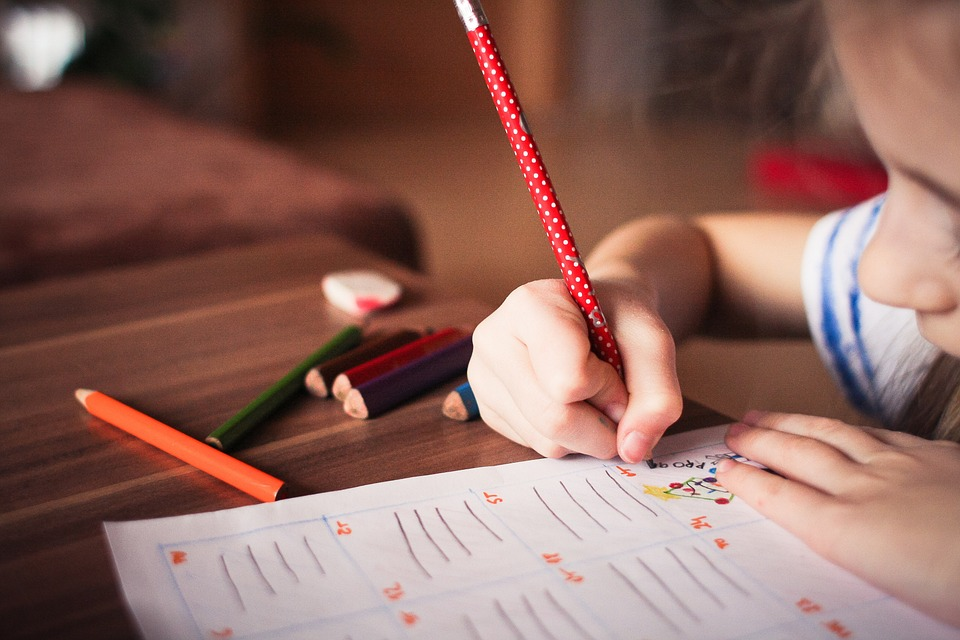
\includegraphics[width=.5\textwidth]{./imgs/img24.jpg}
\caption{Fonte: https://pixabay.com/pt/photos/filho-crian\%c3\%a7a-jogar-estude-cor-865116/}
\end{figure}

\conteudo{A progressão textual é como uma estrada que nos leva de um lugar para
outro, só que no caso dos textos, ela nos leva de uma ideia para outra.
Isso acontece porque os escritores usam palavras e frases para conectar
as ideias que estão escrevendo. Por exemplo, eles podem usar palavras
como ``primeiro'', ``em seguida'' e ``finalmente'' para mostrar a ordem
das coisas que estão acontecendo.

Outra coisa importante que os escritores fazem é usar referências para
falar sobre coisas que já foram mencionadas antes. Isso é chamado de
referência lexical e pronominal. Vamos supor que eu esteja escrevendo um
texto sobre um cachorro e, em vez de dizer ``o cachorro'' toda vez que
eu me referir a ele, eu posso dizer ``ele'' ou ``o animal''. Isso torna
o texto mais fácil de ler e entender.

Além disso, os escritores também podem usar relações de causa e
consequência para explicar por que as coisas acontecem. Por exemplo, se
eu disser ``Eu comi muito doce e fiquei com dor de barriga'', a causa
foi comer muito doce e a consequência foi ter dor de barriga.}

Leia o texto a seguir para entender os mecanismos de progressão textual.

\begin{quote}
\textbf{Um dia de passeio no parque}

Era uma vez uma menina chamada Sofia, que adorava passear no parque.
Certo dia, ela resolveu chamar sua melhor amiga, a Ana, para
acompanhá-la em um delicioso piquenique.

Primeiro, elas foram ao supermercado comprar os alimentos que iriam
levar. Em seguida, caminharam até o parque, que ficava bem perto da casa
da Sofia. Chegando lá, encontraram um lugar muito bonito, com árvores,
flores e um lago com patinhos nadando.

Logo depois de estenderem a toalha no chão, começaram a comer e a
conversar. A Ana contou sobre as férias que passou na praia e a Sofia
falou sobre o livro que estava lendo.

Finalmente, quando já estava ficando tarde, elas recolheram a toalha e
os restos de comida e voltaram para casa, felizes e satisfeitas com o
passeio. Foi um dia muito agradável!
\end{quote}

Nessa história, os mecanismos de progressão textual foram usados para
mostrar a ordem das coisas que aconteceram: primeiro elas foram ao
supermercado, depois caminharam até o parque, em seguida estenderam a
toalha e começaram a comer e conversar, e finalmente recolheram a toalha
e voltaram para casa.

\colorsec{Atividades}

\num{1} Qual é o nome da menina que adora passear no parque?

\linhas{1}
\coment{Sofia.}


\num{2} O que a Sofia resolveu fazer em certo dia?

\linhas{1}
\coment{Ela resolveu chamar sua melhor amiga, a Ana, para acompanhá-la em um
delicioso piquenique.}


\num{3} O que as meninas fizeram primeiro?

\linhas{1}
\coment{Elas foram ao supermercado comprar os alimentos que iriam levar.}


\num{4} Onde ficava o parque que as meninas foram?

\linhas{1}
\coment{O parque ficava bem perto da casa da Sofia.}


\num{5} O que as meninas encontraram quando chegaram ao parque?

\linhas{1}
\coment{Elas encontraram um lugar muito bonito, com árvores, flores e um lago
com patinhos nadando.}


\num{6} O que as meninas fizeram depois de estenderem a toalha no chão?

\linhas{1}
\coment{Elas começaram a comer e a conversar.}


\num{7} Sobre o que a Ana contou para a Sofia?

\linhas{1}
\coment{A Ana contou sobre as férias que passou na praia.}


\num{8} Sobre o que a Sofia falou para a Ana?

\linhas{1}
\coment{A Sofia falou sobre o livro que estava lendo.}


\num{9} O que as meninas fizeram finalmente, quando já estava ficando tarde?

\linhas{1}
\coment{Elas recolheram a toalha e os restos de comida e voltaram para casa.}


\num{10} Como as meninas se sentiram após o passeio?

\linhas{1}
\coment{Elas se sentiram felizes e satisfeitas com o passeio.}


\colorsec{Treino}

\num{1} Leia o texto a seguir para responder à questão.

\begin{quote}
Era uma vez um pobre moleiro que mentiu ao rei, dizendo que sua filha
era capaz de transformar palha em ouro. O rei, que adorava ouro, ordenou
que a moça fosse trazida até ele para realizar o feito.

Assustada, a moça ficou presa em uma sala cheia de palha. Ela chorou,
sem saber o que fazer, até que apareceu um pequeno duende que se
ofereceu para transformar a palha em ouro em troca de algo. A moça
ofereceu seu colar, e o duende realizou o feito.

O rei ficou impressionado com a habilidade da moça e a levou para outra
sala cheia de palha, ordenando que ela transformasse em ouro novamente.
O duende apareceu novamente e, desta vez, pediu o anel da moça em troca
da transformação.

No terceiro dia, a moça foi levada para uma sala ainda maior e cheia de
palha. Ela não tinha mais nada para oferecer ao duende, então ele
sugeriu que ela desse a ele seu primeiro filho quando nascesse. Sem
escolha, a moça aceitou. O rei ficou ainda mais impressionado e decidiu
se casar com a jovem.

Anos depois, a moça deu à luz uma criança, porém, o duende retornou para
pegá-la. A agora rainha implorou por sua liberdade e ofereceu tudo o que
tinha para mantê-lo longe do bebê. O duende sugeriu que, se ela
conseguisse adivinhar seu nome, ele desistiria de seu objetivo.

Assim, a rainha enviou mensageiros por todo o mundo, para descobrir o
nome do duende, mas não teve sucesso. Um dia, andando pela floresta, a
rainha ouviu o duende cantando seu próprio nome, Rumpelstiltskin. Assim,
revelando saber o nome do duende, a rainha pôde manter seu bebê e viver
feliz para sempre.
\end{quote}

Qual foi a consequência da mentira contada pelo pobre moleiro ao rei?

\begin{escolha}
\item A filha do moleiro teve que transformar palha em ouro para o rei.

\item O rei decidiu se casar com a filha do moleiro.

\item O duende apareceu para ajudar a filha do moleiro em troca de algo.

\item A filha do moleiro teve que entregar seu primeiro filho para o duende quando nascesse.
\end{escolha}

\coment{Dificuldade: Médio.

Habilidades SAEB:

- Identificar os mecanismos de progressão textual.

- Identificar os mecanismos de referenciação lexical e pronominal.

- Analisar relações de causa e consequência.

Habilidades BNCC: EF05LP07, EF05LP27.

a) Correto. A mentira do pai da jovem a obrigou a sustentar a mentira
diante do rei, fingindo saber transformar palha em ouro;
b) Incorreto. O rei decidiu se casar em conseqüência do outro fabricado
pelo duende;
c) Incorreto. O duende apareceu buscando o que a moça lhe daria em troca
do favor de salvar sua vida;
d) Incorreto. O acordo de entregar o primeiro filho veio em conseqüência
de a moça não ter mais nada de valor para dar em troca do favor do
doende.}

\num{2} Leia o texto a seguir para responder à questão.

\begin{quote}
Era uma vez um pobre moleiro que mentiu ao rei, dizendo que sua filha
era capaz de transformar palha em ouro. O rei, que adorava ouro, ordenou
que a moça fosse trazida até ele para realizar o feito.

Assustada, a moça ficou presa em uma sala cheia de palha. Ela chorou,
sem saber o que fazer, até que apareceu um pequeno duende que se
ofereceu para transformar a palha em ouro em troca de algo. A moça
ofereceu seu colar, e o duende realizou o feito.

O rei ficou impressionado com a habilidade da moça e a levou para outra
sala cheia de palha, ordenando que ela transformasse em ouro novamente.
O duende apareceu novamente e, desta vez, pediu o anel da moça em troca
da transformação.

No terceiro dia, a moça foi levada para uma sala ainda maior e cheia de
palha. Ela não tinha mais nada para oferecer ao duende, então ele
sugeriu que ela desse a ele seu primeiro filho quando nascesse. Sem
escolha, a moça aceitou. O rei ficou ainda mais impressionado e decidiu
se casar com a jovem.

Anos depois, a moça deu à luz uma criança, porém, o duende retornou para
pegá-la. A agora rainha implorou por sua liberdade e ofereceu tudo o que
tinha para mantê-lo longe do bebê. O duende sugeriu que, se ela
conseguisse adivinhar seu nome, ele desistiria de seu objetivo.

Assim, a rainha enviou mensageiros por todo o mundo, para descobrir o
nome do duende, mas não teve sucesso. Um dia, andando pela floresta, a
rainha ouviu o duende cantando seu próprio nome, Rumpelstiltskin. Assim,
revelando saber o nome do duende, a rainha pôde manter seu bebê e viver
feliz para sempre.
\end{quote}

No texto, como o duende é referido após ter aparecido pela primeira vez?

\begin{escolha}
\item Pelo seu nome verdadeiro, Rumpelstiltskin.

\item Pela sua descrição física, como um pequeno duende.

\item Pela relação com a moça, como aquele que transformou a palha em ouro.

\item Pela sua ação, como aquele que pediu algo em troca pela transformação da palha em ouro.
\end{escolha}

\coment{Dificuldade: Fácil.

Habilidades SAEB:

- Identificar os mecanismos de progressão textual.

- Identificar os mecanismos de referenciação lexical e pronominal.

- Analisar relações de causa e consequência.

Habilidades BNCC: EF05LP07, EF05LP27.

a) Incorreto. O nome do duende é revelado ao término da narrativa;
b) Correto. A aparência do duende é o primeiro elemento que se destaca
na narrativa;
c) Incorreto. A ação do duende vem em um segundo momento, quando, após
ser descrito, oferece ajuda à moça em troca de objetos de valor;
d) Incorreto. O duende já havia sido apresentado ao leitor quando
oferece o acordo de transformar palha em ouro.}

\num{3} Leia o texto a seguir para responder à questão.

\begin{quote}
Era uma vez um pobre moleiro que mentiu ao rei, dizendo que sua filha
era capaz de transformar palha em ouro. O rei, que adorava ouro, ordenou
que a moça fosse trazida até ele para realizar o feito.

Assustada, a moça ficou presa em uma sala cheia de palha. Ela chorou,
sem saber o que fazer, até que apareceu um pequeno duende que se
ofereceu para transformar a palha em ouro em troca de algo. A moça
ofereceu seu colar, e o duende realizou o feito.

O rei ficou impressionado com a habilidade da moça e a levou para outra
sala cheia de palha, ordenando que ela transformasse em ouro novamente.
O duende apareceu novamente e, desta vez, pediu o anel da moça em troca
da transformação.

No terceiro dia, a moça foi levada para uma sala ainda maior e cheia de
palha. Ela não tinha mais nada para oferecer ao duende, então ele
sugeriu que ela desse a ele seu primeiro filho quando nascesse. Sem
escolha, a moça aceitou. O rei ficou ainda mais impressionado e decidiu
se casar com a jovem.

Anos depois, a moça deu à luz uma criança, porém, o duende retornou para
pegá-la. A agora rainha implorou por sua liberdade e ofereceu tudo o que
tinha para mantê-lo longe do bebê. O duende sugeriu que, se ela
conseguisse adivinhar seu nome, ele desistiria de seu objetivo.

Assim, a rainha enviou mensageiros por todo o mundo, para descobrir o
nome do duende, mas não teve sucesso. Um dia, andando pela floresta, a
rainha ouviu o duende cantando seu próprio nome, Rumpelstiltskin. Assim,
revelando saber o nome do duende, a rainha pôde manter seu bebê e viver
feliz para sempre.
\end{quote}

Qual foi a causa para a rainha ter que adivinhar o nome do duende?

\begin{escolha}
\item O rei ordenou que a rainha descobrisse o nome do duende.

\item A rainha fez um acordo com o duende para manter seu bebê.

\item A rainha queria provar sua inteligência ao duende.

\item A rainha queria se vingar do duende por tê-la ameaçado.
\end{escolha}

\coment{Dificuldade: Médio.

Habilidades SAEB:

- Identificar os mecanismos de progressão textual.

- Identificar os mecanismos de referenciação lexical e pronominal.

- Analisar relações de causa e consequência.

Habilidades BNCC: EF05LP07, EF05LP27.

a) Incorreto. O rei nada sabe sobre o duende, segundo a narrativa;
b) Correto. O duende propõe que a rainha descubra seu nome como condição
para quebrar o acordo;
c) Incorreto. O interesse da rainha em buscar o nome do duende era
manter seu bebê;
d) Incorreto. A rainha busca os meios de romper o acordo com o duende,
pois não deseja se separar da criança.}

\chapter{Simulado 1}

\num{1} Leia o texto a seguir e responda à pergunta:

\begin{quote}
\textbf{Novo método de reciclagem pode viabilizar a economia circular dos plásticos}

Resíduos plásticos se espalham aceleradamente pelo planeta causando
danos à biodiversidade, à saúde humana, à economia, e ao equilíbrio
climático. Diante desse desafio crescente, um método inovador --
descrito, em outubro, num artigo publicado pela revista Science --
aponta um promissor caminho de desenvolvimento tecnológico. A abordagem
combina processos biológicos e químicos para simplificar e aumentar a
eficiência da reciclagem de misturas de vários tipos de plástico.

{[}...{]}.

\fonte{Fonte:
https://www.ipea.gov.br/cts/pt/central-de-conteudo/noticias/noticias/329-novo-metodo-de-reciclagem-pode-viabilizar-a-economia-circular-dos-plasticos.
Acesso em 25/02/2023.}
\end{quote}

De acordo com o texto, a nova forma de reciclagem

\begin{escolha}
\item só pode ser utilizada com papel.

\item não é muito prática.

\item aumenta a eficiência do processo.

\item produz maiores quantidades de lixo.
\end{escolha}

\coment{Dificuldade: Média.

Saeb: Localizar informação explícita. BNCC: (EF15LP03) Localizar
informações explícitas em textos.

a) Incorreta. O texto menciona somente o plástico;
b) Incorreta. O texto não fala sobre a praticidade do processo;
c) Correta. O texto afirma explicitamente que o novo procedimento
aumenta a eficiência da reciclagem;
d) Incorreta. O texto parte de um pressuposto oposto.}

\num{2} Leia o texto a seguir e responda à pergunta:

\begin{quote}
\textbf{João e o Pé de Feijão}

Era uma vez garoto chamado João, que morava com sua mãe em uma pequena
casa na floresta. João e sua mãe eram muito pobres e tinham dificuldades
para conseguir dinheiro e comida suficientes para sobreviver.

Um dia, João foi até a cidade para vender a única vaca da família. No
caminho, ele encontrou um homem misterioso que lhe ofereceu cinco
feijões mágicos em troca da vaca. João aceitou e voltou para casa com os
feijões

{[}...{]}.
\end{quote}

Na narrativa acima, as personagens citadas são

\begin{escolha}
\item João, sua mãe, a vaca da família e o homem misterioso.

\item João e sua mãe.

\item João e o homem misterioso.

\item João e os feijões.
\end{escolha}

\coment{Dificuldade: Fácil.

Saeb: Identificar elementos constitutivos de textos narrativos. BNCC:
(EF35LP26) Ler e compreender, com certa autonomia, narrativas ficcionais
que apresentem cenários e personagens, observando os elementos da
estrutura narrativa: enredo, tempo, espaço, personagens, narrador e a
construção do discurso indireto e discurso direto.

a) Correta. Ao longo do texto encontramos essas quatro personagens;
b) Incorreta. Não foram mencionados a vaca e o homem misterioso na
alternativa;
c) Incorreta. Não foram mencionadas a mãe de João e a vaca na
alternativa;
d) Incorreta. Os feijões não podem ser considerados personagens.}

\num{3} Leia o texto a seguir e responda à pergunta:

\begin{quote}
\textbf{Vulcão das Canárias abre caminho para a previsão das erupções}

Graças a novas ferramentas e descobertas, os vulcanologistas buscam um
modelo que permita estimar quando os fenômenos surgirão e durante quanto
tempo. Um artigo da `Science' discute um método para calcular o período
de reativação, citando como exemplo o que aconteceu em Cumbre Vieja
(Espanha).

{[}...{]}.

\fonte{Fonte:
https://brasil.elpais.com/ciencia/2021-12-03/vulcao-das-canarias-abre-caminho-para-a-previsao-das-erupcoes.html.
Acesso em 25/02/2023.}
\end{quote}

A notícia reproduzida acima discute

\begin{escolha}
\item uma recente erupção de um vulcão localizado no Havaí.

\item as atividades realizadas por vulcanologistas.

\item a ciência espanhola.

\item a busca de cientistas por novas formas de prever uma erupção.
\end{escolha}

\coment{Dificuldade: Fácil.

Saeb: Analisar elementos constitutivos de gêneros textuais diversos.
BNCC: (EF35LP16) Identificar e reproduzir, em notícias, manchetes, lides
e corpo de notícias simples para público infantil e cartas de reclamação
(revista infantil), digitais ou impressos, a formatação e diagramação
específica de cada um desses gêneros, inclusive em suas versões orais.

a) Incorreta. O texto menciona apenas um vulcão na Espanha;
b) Incorreta. O texto não entra em detalhes a respeito dessas
atividades;
c) Incorreta. O texto apenas menciona um vulcão espanhol;
d) Correta. O texto trata da busca por novas maneiras de realizar essa
previsão.}

\num{4} Leia o texto a seguir e responda à pergunta:

\begin{quote}
\textbf{Controle e prevenção do desmatamento e dos incêndios florestais}

Prevenir e combater o desmatamento ilegal e os incêndios florestais num
país em desenvolvimento e de dimensões continentais como o Brasil não é
uma tarefa fácil. Principalmente na Amazônia Legal, que corresponde a
cerca de 61\% do território nacional e possui um patrimônio ambiental
com enorme potencial econômico, ainda pouco explorado.

{[}...{]}

São necessárias, portanto, medidas positivas que possam influenciar
novas dinâmicas e modelos produtivos sustentáveis como alternativa à
supressão da vegetação nativa, trazendo os diferentes setores da
sociedade para atuar em conjunto no combate ao desmatamento ilegal.

{[}...{]}.

\fonte{Fonte:
https://www.gov.br/mma/pt-br/assuntos/servicosambientais/controle-de-desmatamento-e-incendios-florestais.
Acesso em 25/02/2023.}
\end{quote}

O texto acima procura convencer o leitor

\begin{escolha}
\item da necessidade de controlarmos e prevenirmos os incêndios florestais.

\item da necessidade de expandirmos o patrimônio natural brasileiro.

\item das belezas da flora brasileira.

\item dos perigos da diminuição do território natural brasileiro.
\end{escolha}

\coment{Dificuldade: Fácil.

Saeb: Analisar o uso de recursos de persuasão em textos verbais e/ou
multimodais.. BNCC: (EF05LP20) Analisar a validade e força de argumentos
em argumentações sobre produtos de mídia para público infantil (filmes,
desenhos animados, HQs, games etc.), com base em conhecimentos sobre os
mesmos.

a) Correta. O texto expõe formas para manutenção da natureza brasileira;
b) Incorreta. O texto não trabalha com a possibilidade de expansão;
c) Incorreta. O texto não procura convencer o leitor dessa
característica;
d) Incorreta. O texto apenas constata essa diminuição.}

\num{5} Leia o trecho do poema a seguir e responda à questão:

\begin{quote}
\textbf{Rosa Murcha}

Esta rosa desbotada\\
Já tantas vezes beijada,\\
Pálido emblema de amor;\\
É uma folha caída\\
Do livro da minha vida,\\
Um canto imenso de dor!\\
{[}...{]}

\fonte{DE ABREU, Casimiro. Rosa Murcha. In: \emph{As Primaveras}.
Rio de Janeiro: Typ. de Paula Brito, 1859.}
\end{quote}

A estrofe acima apresenta as rimas

\begin{escolha}
\item desbotada/beijada e folha/livro.

\item amor/dor e rosa/desbotada.

\item caída/vida, amor/dor e livro/canto.

\item desbotada/beijada, caída/vida e amor/dor.
\end{escolha}

\coment{Dificuldade: Média.

Saeb: Analisar o uso de recursos de persuasão em textos verbais e/ou
multimodais.. BNCC: (EF35LP27) - Ler e compreender, com certa autonomia,
textos em versos, explorando rimas, sons e jogos de palavras, imagens
poéticas (sentidos figurados) e recursos visuais e sonoros.

a) Incorreta. O par de palavras folha/livro não constitui uma rima;
b) Incorreta. O par de palavras rosa/desbotada não constitui uma rima;
c) Incorreta. O par de palavras livro/canto não constitui uma rima;
d) Correta. A estrofe apresenta as rimas citadas.}

\num{6} Leia o trecho a seguir e responda à pergunta:

\begin{quote}
Um destes dias, leva por aí algum tiro para lhe botar juízo na
\emph{cachola} {[}...{]} Nem sempre há de ter cartas de irmão para
sair-se bem da \emph{rascada}.

\fonte{TAUNAY, Visconde de. Inocência. Disponível:
http://objdigital.bn.br/Acervo\_Digital/livros\_eletronicos/inocencia.pdf.
Acesso em: 26 fev. 2023. }
\end{quote}

Os termos destacados também significam, respectivamente

\begin{escolha}
\item cachoeira e rasgo.

\item cabeça e enrascada.

\item caixa e risco.

\item cacho e risco.
\end{escolha}

\coment{Dificuldade: Difícil.

Saeb: Identificar as variedades linguísticas em textos. BNCC: (EF35LP22)
- Perceber diálogos em textos narrativos, observando o efeito de sentido
de verbos de enunciação e, se for o caso, o uso de variedades
linguísticas no discurso direto.

a) Incorreta. As palavras mencionadas se assemelham apenas foneticamente
às variações no texto;
b) Correta. As palavras mencionadas são variações linguísticas de cabeça
e enrascada;
c) Incorreta. As palavras mencionadas se assemelham apenas foneticamente
às variações no texto;
d) Incorreta. As palavras mencionadas se assemelham apenas foneticamente
às variações no texto.}

\num{7} Leia o texto a seguir e responda à pergunta:

\begin{quote}
\textbf{Por que cada vez mais pessoas estão vivendo até os 100 anos?}

Comemorar 100 aniversários é ainda mais difícil. Nos Estados Unidos,
um estudo de longo prazo da Universidade de Boston estimou que apenas 1
em cada 5 milhões de americanos atinge o estágio "supercentenário" ---
quando se ultrapassa os 110 anos.

Essa taxa, porém, vem aumentando. Em 2010, os pesquisadores americanos
contavam cerca de 60 a 70 pessoas nessa faixa etária. Em 2017, esse
número havia se expandido para 150.

Os "supercentenários" naturalmente atraem muita atenção dos cientistas
que estudam o envelhecimento humano.

\fonte{Fonte: https://www.bbc.com/portuguese/geral-62120822.
Acesso em 25/02/2023. }
\end{quote}

No título do texto acima, o ponto de interrogação indica

\begin{escolha}
\item o destaque de uma ideia.

\item a divisão entre duas frases.

\item o fim de uma frase.

\item uma pergunta.
\end{escolha}

\coment{Dificuldade: Fácil

Saeb: Analisar os efeitos de sentido decorrentes do uso da pontuação.
BNCC: (EF05LP04) Diferenciar, na leitura de textos, vírgula, ponto e
vírgula, dois-pontos e reconhecer, na leitura de textos, o efeito de
sentido que decorre do uso de reticências, aspas, parênteses.

a) Incorreta. O ponto de exclamação é usada para destacar ideias;
b) Incorreta. A vírgula é usada para dividir duas frases;
c) Incorreta. O ponto final é usado para marcar o final de uma frase;
d) Correta. O ponto de interrogação é usado para marcar perguntas.}

\chapter{Simulado 2}

\num{1} Leia o trecho a seguir e responda à pergunta:

\begin{quote}
{[}...{]}

D. CARLOTA --- Não sei nada; sou uma tagarela, que o senhor obrigou a
dar por paus e por pedras; mas, como é a última vez que nos vemos, não
importa. Agora, passe bem.

CAVALCANTE: Adeus, D. Carlota!

D. CARLOTA: Adeus, doutor!

CAVALCANTE: Adeus. (Dá um passo para a porta do fundo). Talvez eu vá a
Atenas; não fuja se me vir vestido de frade.

{[}...{]}.

\fonte{ASSIS, Joaquim Maria Machado de. \emph{Não Consultes Médico}.
Disponível em:
https://machado.mec.gov.br/obra-completa-lista/item/download/66\_390921fb4791464b4885563dc04a042c.
Acesso em 26/02/2023.}
\end{quote}

No texto dramático acima, a ação a ser desempenhada pelo ator é descrita
no trecho

\begin{escolha}
\item ``Adeus, doutor!''

\item ``Talvez eu vá a Atenas;''

\item ``(Dá um passo para a porta do fundo)''.

\item ``Agora, passe bem.''
\end{escolha}

\coment{Dificuldade: Difícil

Saeb: Identificar as marcas de organização de textos dramáticos. BNCC:
(EF35LP24) Identificar funções do texto dramático (escrito para ser
encenado) e sua organização por meio de diálogos entre personagens e
marcadores das falas das personagens e de cena.

a) Incorreta. O trecho faz parte de um diálogo;
b) Incorreta. O trecho faz parte de um diálogo;
c) Correta. O trecho contém instruções de cena específicas para o ator;
d) Incorreta. O trecho faz parte de um diálogo.}

\num{2} Leia o trecho a seguir e responda à pergunta:

\begin{quote}
{[}...{]} Em casa, ficaram querendo bem a Escobar; a mesma prima
Justina achou que era um moço muito apreciável, apesar... --- Apesar de
quê? perguntou-lhe José Dias, vendo que ela não acabava a frase. Não
teve resposta, nem podia tê-la; prima Justina provavelmente não viu
defeito claro ou importante no nosso hóspede; {[}...{]}.

\fonte{ASSIS, Joaquim Maria Machado de. \emph{Dom Casmurro.}
Disponível em:
https://machado.mec.gov.br/obra-completa-lista/item/download/13\_7101e1a36cda79f6c97341757dcc4d04.
Acesso em 26/02/2023.}
\end{quote}

O trecho reproduzido acima apresenta o verbo de enunciação

\begin{escolha}
\item perguntar.

\item ficar.

\item ver.

\item poder.
\end{escolha}

\coment{Dificuldade: Média

Saeb: Analisar os efeitos de sentido de verbos de enunciação. BNCC:
(EF05LP10) Ler e compreender, com autonomia, anedotas, piadas e cartuns,
dentre outros gêneros do campo da vida cotidiana, de acordo com as
convenções do gênero e considerando a situação comunicativa e a
finalidade do texto.

a) Correta. O verbo perguntar está relacionado a uma fala da personagem;
b) Incorreta. O verbo ficar não é um verbo de enunciação;
c) Incorreta. O verbo ver não faz referência a uma fala das personagens;
d) Incorreta. O verbo poder não remete a um diálogo.}

\num{3} Leia o texto a seguir e responda à pergunta:

\begin{quote}
\textbf{Nasa consegue registrar grandes impactos de corpos celestes em Marte}

Uma sonda espacial da Nasa testemunhou a formação de uma enorme
cratera em Marte --- a maior do Sistema Solar já capturada no momento de
sua abertura.

O impacto causado por um corpo celeste do tamanho de uma van abriu um
buraco de 150 m de largura no planeta vermelho, lançando detritos a até
35 km de distância.

Os cientistas detectaram o evento usando o sismógrafo da sonda InSight,
da agência espacial americana, que captou as vibrações do solo.

{[}...{]}.

\fonte{Fonte:
https://www.bbc.com/portuguese/internacional-63424518. Acesso em
26/02/2023.}
\end{quote}

O tema do texto acima refere-se

\begin{escolha}
\item a impactos observados na superfície de Marte.

\item ao corpo celeste que cairá na Terra.

\item à construção da sonda InSight.

\item às vibrações do solo detectadas na Terra.
\end{escolha}

\coment{Dificuldade: Média

Saeb: Analisar os efeitos de sentido de verbos de enunciação. BNCC:
(EF05LP10) Ler e compreender, com autonomia, anedotas, piadas e cartuns,
dentre outros gêneros do campo da vida cotidiana, de acordo com as
convenções do gênero e considerando a situação comunicativa e a
finalidade do texto.

a) Correta. O texto fala sobre a observação de impactos ocorridos em
Marte;
b) Incorreta. O texto cita somente objetos que caíram em Marte;
c) Incorreta. O texto não faz menção à construção da sonda;
d) Incorreta. As vibrações foram detectadas em Marte.}

\num{4} Leia os trechos a seguir e responda à pergunta:

\begin{quote}
{[}...{]} Quis tapar-lhe a boca. José Dias viu no meu rosto algum
sinal diferente da expressão habitual, e perguntou-me com interesse

-- Que é, Bentinho?

{[}...{]}

\fonte{ASSIS, Joaquim Maria Machado de. \emph{Dom Casmurro.}
Disponível em:
https://machado.mec.gov.br/obra-completa-lista/item/download/13\_7101e1a36cda79f6c97341757dcc4d04.
Acesso em 26/02/2023.}
\end{quote}

\begin{quote}
José Dias (olhando com interesse): Que é, Bentinho?

\fonte{Adaptado de ASSIS, Joaquim Maria Machado de. \emph{Dom
Casmurro.} Disponível em:
https://machado.mec.gov.br/obra-completa-lista/item/download/13\_7101e1a36cda79f6c97341757dcc4d04.
Acesso em 26/02/2023.}
\end{quote}

A partir da comparação entre os dois trechos acima, podemos dizer que a
principal diferença entre o texto narrativo e o texto dramático reside

\begin{escolha}
\item no uso de personagens.

\item na temática explorada.

\item na presença de um narrador.

\item no tipo de linguagem explorado.
\end{escolha}

\coment{Dificuldade: Média

Saeb: Reconhecer diferentes gêneros textuais. BNCC: (EF35LP29)
Identificar, em narrativas, cenário, personagem central, conflito
gerador, resolução e o ponto de vista com base no qual histórias são
narradas, diferenciando narrativas em primeira e terceira pessoas.

a) Incorreta. Ambos os tipos de texto apresentam personagens;
b) Incorreta. Os dois tipos de texto podem apresentar a mesma temática;
c) Correta. O texto narrativo, ao contrário do dramático, apresenta um
narrador;
d) Incorreta. Os registros linguísticos podem ser os mesmos nos dois
tipos de texto.}

\num{5} Leia o texto a seguir e responda à pergunta:

\begin{quote}
\textbf{Superlaboratório Sirius atrai atenção de cientistas da
Argentina, Grã-Bretanha, Alemanha e EUA}

Acelerador de partículas em Campinas (SP) recebeu propostas de
pesquisa de diversas instituições brasileiras e internacionais.
Trabalhos selecionados serão agendados a partir de março.

{[}...{]} o Sirius surge como uma alternativa, já que a máquina é
mundialmente \textbf{competitiva}, possibilita diferentes tipos de
análise com qualidade e com rapidez" {[}...{]}.

\fonte{Fonte:
https://g1.globo.com/sp/campinas-regiao/noticia/2023/02/17/superlaboratorio-sirius-atrai-atencao-de-cientistas-da-argentina-gra-bretanha-alemanha-e-eua.ghtml.
Acesso em 26/02/2023.}
\end{quote}

O adjetivo destacado revela, acerca do laboratório, uma visão

\begin{escolha}
\item duvidosa.

\item neutra.

\item positiva.

\item negativa.
\end{escolha}

\coment{Dificuldade: Fácil

Saeb: Analisar os efeitos de sentido decorrentes do uso dos adjetivos.
BNCC: Não há correspondência.

a) Incorreta. O adjetivo revela uma visão clara a respeito do assunto;
b) Incorreta. Uma visão neutra a respeito do assunto não utilizaria um
adjetivo positivo;
c) Correta. O adjetivo ``competitiva'' revela um atributo positivo;
d) Incorreta. O adjetivo atribui um sentido oposto.}

\num{6} Leia o texto a seguir e responda à pergunta:


\begin{tabular}{|ll|}
\hline
\multicolumn{2}{|c|}{\begin{tabular}[c]{@{}c@{}}Número de alunos matriculados na 5.ª série\\ Estado de São Paulo\end{tabular}} \\ \hline
\multicolumn{1}{|l|}{Meninas} & 2.809 \\ \hline
\multicolumn{1}{|l|}{Meninos} & 3.164 \\ \hline
\end{tabular}

\begin{figure}[htpb!]
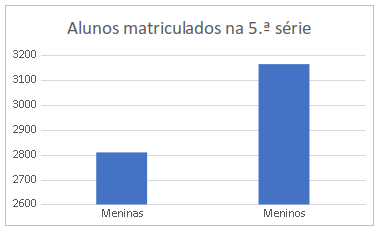
\includegraphics[width=.5\textwidth]{./imgs/chart4.png}
\end{figure}

\fonte{Adaptado de http://www.educacao.sp.gov.br/a2sitebox/arquivos/documentos/967.pdf. Acesso em 26/02/2023.}

De acordo com a tabela e o gráfico acima, podemos chegar à conclusão de
que

\begin{escolha}
\item O número de meninos e meninas matriculados é desconhecido.

\item O número de meninos e meninas matriculados é igual.

\item O número de meninas matriculadas é maior que o de meninos.

\item O número de meninos matriculados é maior que o de meninas.
\end{escolha}

\coment{Dificuldade: Fácil

Saeb: Analisar informações apresentadas em gráficos, infográficos ou
tabelas. BNCC (EF05LP23): Comparar informações apresentadas em gráficos
ou tabelas.

a) Incorreta. A tabela e o gráfico mostram claramente a informação
requisitada;
b) Incorreta. A tabela e o gráfico não demonstram igualdade;
c) Incorreta. A tabela e o gráfico implicam uma conclusão oposta;
d) Correta. A tabela e o gráfico confirmam essa informação.}

\num{7} Leia o texto a seguir e responda à pergunta:

\begin{quote}
O mini-helicóptero Ingenuity, da Nasa, entrou para o "Guinness World
Records" com o voo mais longo realizado na superfície marciana.

{[}...{]}

O Ingenuity, que se assemelha a um drone, pesa 1,8kg e chegou a Marte
dobrado e acoplado à parte inferior do Perseverance, robô da Nasa que
pousou no planeta em fevereiro de 2021.

{[}...{]}

``Temos confiança de que podemos contar com o Perseverance para trazer
as amostras de volta e adicionamos os helicópteros como uma espécie de
plano B'', disse Gramling.

{[}...{]}.

\fonte{Fonte:
https://g1.globo.com/ciencia/noticia/2023/02/14/helicoptero-da-nasa-entra-para-o-guinness-world-records-com-o-voo-mais-longo-em-marte.ghtml.
Acesso em: 26/02/2023.}
\end{quote}

No texto acima, a opinião do especialista é

\begin{escolha}
\item colocada entre aspas.

\item descrita ao longo dos parágrafos.

\item suprimida do texto.

\item colocada no título.
\end{escolha}

\coment{Dificuldade: Média

Saeb: Distinguir fatos de opiniões em textos. BNCC (EF05LP16): Comparar
informações sobre um mesmo fato veiculadas em diferentes mídias e
concluir sobre qual é mais confiável e por quê.

a) Correta. A fala do especialista é reproduzida entre aspas;
b) Incorreta. A fala do especialista surge somente ao final do texto;
c) Incorreta. A fala do especialista surge ao final do texto;
d) Correta. O título apresenta o tema do texto.}

\chapter{Simulado 3}

\num{1} Leia o texto a seguir e responda à pergunta:

\begin{quote}
\textbf{Cientistas usam câmera especial para mostrar para-raios em ação}

Com uma câmera de vídeo ultrarrápida, e o trunfo de estar no lugar
certo no momento certo, o físico Marcelo Saba, pesquisador do Instituto
Nacional de Pesquisas Espaciais (Inpe), e o doutorando Diego Rhamon
obtiveram uma imagem inédita da descarga de um raio, mostrando detalhes
de sua conexão com vários para-raios localizados nas imediações.

{[}...{]}.

\fonte{Fonte:
https://veja.abril.com.br/ciencia/cientistas-usam-camera-especial-para-mostrar-para-raios-em-acao/.
Acesso em 26/02/2023.}
\end{quote}

A partir do texto reproduzido acima, podemos chegar à conclusão de que

\begin{escolha}
\item os pesquisadores não foram bem-sucedidos.

\item descargas de raios não podem ser filmadas.

\item descargas de raios são muito rápidas para serem filmadas com câmeras normais.

\item tempestades de raios são muito perigosas.
\end{escolha}

\coment{Dificuldade: Difícil

Saeb: Inferir informações implícitas em textos. BNCC (EF35LP04): Inferir
informações implícitas nos textos lidos.

a) Incorreta. O texto menciona que os pesquisadores foram bem-sucedidos;
b) Incorreta. O texto descreve como os pesquisadores foram capazes de
filmar as descargas elétricas;
c) Correta. O fato de os pesquisadores usarem uma câmera ultrarrápida
confirma essa informação;
d) Incorreta. O texto não menciona o perigo dos raios.}

\num{2} Leia o texto a seguir e responda à pergunta:

\begin{quote}
\textbf{Cosmonautas presos na Estação Espacial Internacional voltam em
setembro}

Tripulação russa deve encerrar uma missão espacial em março, mas não
pode deixar o espaço devido a um acidente na espaçonave MS-22.

{[}...{]}

O acidente envolveu o sistema de resfriamento da cápsula Soyuz MS-22,
que começou a vazar há dois meses. {[}...{]} Por esse motivo a equipe
não consegue deixar a Estação Espacial Internacional \textbf{(ISS, na
sigla em inglês)}. A previsão de retorno ficou para setembro deste ano,
e envolverá a substituição da parte danificada.

{[}...{]}.

\fonte{Fonte:
https://veja.abril.com.br/ciencia/cosmonautas-presos-na-estacao-espacial-internacional-voltam-em-setembro/.
Acesso em 26/02/2023.}
\end{quote}

O trecho destacado entre parênteses cumpre a função de

\begin{escolha}
\item explicar uma informação previamente exposta.

\item concluir a frase.

\item pontuar uma dúvida.

\item destacar uma informação.
\end{escolha}

\coment{Dificuldade: Média

Saeb: Analisar os efeitos de sentido decorrentes do uso da pontuação.
BNCC (EF05LP04): Diferenciar, na leitura de textos, vírgula, ponto e
vírgula, dois-pontos e reconhecer, na leitura de textos, o efeito de
sentido que decorre do uso de reticências, aspas, parênteses.

a) Correta. Os parênteses são utilizados para explicar a sigla da
Estação Espacial;
b) Incorreta. O ponto final é usado para concluir uma frase;
c) Incorreta. O ponto de interrogação é usado para marcar uma dúvida;
d) Incorreta. O ponto de exclamação é usado para destacar uma
informação.}

\num{3} Leia o texto a seguir e responda à pergunta:

\begin{quote}
{[}...{]} Na conversa de \textbf{anteontem} com Rita esqueceu-me dizer
a parte relativa a minha mulher, que lá está enterrada em Viena. Pela
segunda vez falou-me em transportá-la para o nosso jazigo. Novamente lhe
disse que estimaria muito estar perto dela, mas que, em minha opinião,
os mortos ficam bem onde caem; redarguiu-me que estão muito melhor com
os seus.

{[}...{]}.

\fonte{ASSIS, Joaquim Maria Machado de. \emph{Memorial de Aires}.
Disponível em:
https://machado.mec.gov.br/obra-completa-lista/item/download/10\_3b418d3289f560235fccf338378de5bf.
Acesso em 26/02/2023.}
\end{quote}

O advérbio destacado no trecho acima indica

\begin{escolha}
\item o local em que um determinado fato ocorreu.

\item a negação de um determinado fato.

\item o modo como um determinado fato ocorreu.

\item o momento em que um determinado fato ocorreu.
\end{escolha}

\coment{Dificuldade: Fácil

Saeb: Analisar os efeitos de sentido decorrentes do uso dos advérbios.
Não há correspondência.

a) Incorreta. Não se trata de um advérbio de lugar;
b) Incorreta. Não se trata de um advérbio de negação;
c) Incorreta. Não se trata de um advérbio de modo;
d) Correta. Trata-se de um advérbio de tempo.}

\num{4} Leia o trecho a seguir e responda à pergunta:

\begin{quote}
\textbf{Orações}

{[}...{]}

As doces falas de tua alma santa\\
Valem mais do que eu valho, oh querubim!\\
Quando rezares por teu mano, à noite,\\
Não te esqueças também -- reza por mim!''

\fonte{ABREU, Casimiro de. Orações. In: \emph{Cantos de Tristeza e
Saudade.} Paris: Casa Editorial Franco-Ibero-Americana,
19?.}
\end{quote}

A estrofe reproduzida acima reflete um tema de

\begin{escolha}
\item indiferença.

\item tristeza.

\item raiva.

\item amor.
\end{escolha}

\coment{Dificuldade: Fácil

Saeb: Analisar a construção de sentidos de textos em versos com base em
seus elementos constitutivos. BNCC (EF35LP31): Identificar, em textos
versificados, efeitos de sentido decorrentes do uso de recursos rítmicos
e sonoros e de metáforas.

a) Incorreta. A estrofe exibe grande intensidade de emoções;
b) Incorreta. A estrofe não apresenta sentimentos tristes;
c) Incorreta. A estrofe apresenta sentimentos positivos;
d) Correta. A estrofe descreve o amor romântico em um pedido de orações.}

\num{5} Leia o texto a seguir e responda à questão:

\begin{quote}
\textbf{Astrônomos identificam misterioso objeto celeste e descobrem
galáxia}

Existe um objeto celeste misterioso e extremamente remoto, com um
sexto do tamanho do nosso, situado em um universo ainda ``jovem'', com
cerca de 2 bilhões de anos, tão escuro que é praticamente invisível,
mesmo para os instrumentos mais avançados disponíveis no momento
{[}...{]}.

O corpo escuro e compacto, oculto por grandes quantidades de poeira
estelar, é uma galáxia jovem que forma estrelas em uma velocidade
surpreendente (cerca de 1000 vezes a taxa da Via Láctea).

{[}...{]}.
\end{quote}

Os dois parágrafos reproduzidos acima estabelecem uma relação de

\begin{escolha}
\item redundância.

\item conclusão.

\item oposição.

\item adição.
\end{escolha}

\coment{Dificuldade: Difícil

Saeb: Identificar os mecanismos de progressão textual. BNCC (EF05LP07):
Identificar, em textos, o uso de conjunções e a relação que estabelecem
entre partes do texto: adição, oposição, tempo, causa, condição,
finalidade.

a) Incorreta. O segundo parágrafo traz novas informações, não sendo,
portanto, redundante;
b) Incorreta. O segundo parágrafo não conclui o assunto tratado no
texto;
c) Incorreta. Os dois parágrafos tratam do mesmo assunto por meio de uma
mesma perspectiva;
d) Correta. O segundo parágrafo adiciona novas informações ao tema
discutido anteriormente.}

\num{6} Analise o cartaz abaixo e responda à pergunta:

\begin{figure}[htpb!]
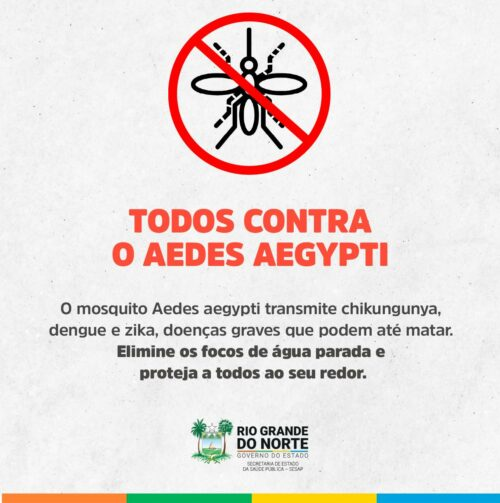
\includegraphics[width=.5\textwidth]{./imgs/img25.jpg}
\caption{Fonte: https://portalcovid19.saude.rn.gov.br/noticias/sesap-orienta-populacao-para-prevencao-a-dengue-chikungunya-e-zika/. Acesso em 26/02/2023.}
\end{figure}

O uso do cartaz acima em um texto contra a dengue cumpre a função de

\begin{escolha}
\item negar o que foi escrito.

\item fortalecer o argumento pelo combate ao mosquito.

\item substituir o que foi escrito.

\item estimular a criação de focos do mosquito.
\end{escolha}

\coment{Dificuldade: Fácil

Saeb: Analisar os efeitos de sentido de recursos multissemiótico em
textos que circulam em diferentes suportes. BNCC (EF05LP20): Analisar a
validade e força de argumentos em argumentações sobre produtos de mídia
para público infantil (filmes, desenhos animados, HQs, games etc.), com
base em conhecimentos sobre os mesmos.

a) Incorreta. O cartaz cumpre a função oposta;
b) Correta. O artifício visual reforça o ponto de vista construído no
texto;
c) Incorreta. O cartaz cumpre a função de complementar, e não
substituir;
d) Incorreta. O cartaz defende o ponto de vista oposto.}

\num{7} Leia o texto a seguir e responda à pergunta:

\begin{quote}
\textbf{Manter caderneta de vacinação em dia é fundamental para prevenir
doenças}

{[}...{]}

Para além das vacinas contra a Covid-19 e Influenza, diversas outras que
compõem o calendário nacional de vacinação estão disponíveis nas salas
de vacina, localizadas nas unidades básicas de saúde (UBS). É importante
que a população se atente para a necessidade de manter em dia o esquema
de vacinação como forma de prevenir doenças para as quais já existe
imunização.

Segundo a enfermeira da área técnica de imunização da Secretaria de
Saúde, Fernanda Ledes, todas as vacinas preconizadas pelo Programa
Nacional de Imunizações (PNI), do Ministério da Saúde, e que fazem parte
do calendário nacional são extremamente importantes e devem ser
realizadas nas faixas etárias {[}...{]}. ``A vacina é uma medida
preventiva, e não curativa. Devemos nos vacinar justamente para que as
doenças não circulem entre nós'', alerta.

{[}...{]}.

\fonte{Fonte:
https://www.saude.df.gov.br/web/guest/w/manter-caderneta-de-vacinacao-em-dia-e-fundamental-para-prevenir-doencas.
Acesso em 26/02/2023.}
\end{quote}

Selecione a seguir um dos argumentos utilizados no texto para defender a
vacinação:

\begin{escolha}
\item Devemos nos vacinar para que os programas de imunização sejam expandidos.

\item A vacinação impede que as doenças circulem.

\item O processo de fabricação dos imunizantes será conhecido pela população.

\item É importante nos vacinarmos apenas no calendário de imunização.
\end{escolha}

\coment{Dificuldade: Média

Saeb: Julgar a eficácia de argumentos em textos. BNCC (EF05LP20):
Analisar a validade e força de argumentos em argumentações sobre
produtos de mídia para público infantil (filmes, desenhos animados, HQs,
games etc.), com base em conhecimentos sobre os mesmos.

a) Incorreta. O texto não menciona a expansão desses programas;
b) Correta. O texto cita explicitamente esse argumento;
c) Incorreta. O texto não trata do processo de fabricação das vacinas;
d) Incorreta. O texto menciona o calendário, mas não afirma que podemos
nos vacinar apenas durante sua vigência.}

\chapter{Simulado 4}

\num{1} Leia os textos a seguir e responda à pergunta:

\begin{quote}
\textbf{Texto I: Nova imagem da Via Láctea mostra mais de 3 bilhões de
estrelas}

Endereço do Sistema Solar, a Via Láctea contém centenas de bilhões de
estrelas, regiões cintilantes de formação estelar e enormes nuvens
escuras de poeira e gás. Catalogar esses objetos é uma tarefa trabalhosa
e longa, mas o segundo conjunto de dados da Pesquisa com Câmera de
Energia Escura (DECaPS2) revelou recentemente um número impressionante
desses corpos celestes em detalhes nunca antes vistos. {[}...{]}.

{[}...{]}

Apesar dos desafios, os astrônomos foram capazes de espiar através de
grande parte da poeira que absorve a luz usando equipamentos de
infravermelho. Os pesquisadores também usaram uma abordagem inovadora de
processamento de dados, que lhes permitiu prever melhor o fundo por trás
de cada estrela.

\fonte{Fonte:
https://veja.abril.com.br/ciencia/nova-imagem-da-via-lactea-mostra-mais-de-3-bilhoes-de-estrelas/.
Acesso em 26/02/2023.}
\end{quote}

\begin{quote}
\textbf{Texto II: Levantamento inédito da Via Láctea revela 3,3 bilhões
de objetos celestes}

Astrônomos divulgaram um novo levantamento sobre os objetos celestes
que compõem a Via Láctea. Obtidos por meio do Plano Galáctico com a
Câmera de Energia Escura (DECaPS2), os dados inéditos apresentam
impressionantes 3,32 bilhões de formações que incluem estrelas, regiões
cintilantes de formação estelar e enormes nuvens escuras de poeira e
gás.

{[}...{]}

``Uma das principais razões para o sucesso do DECaPS2 é que simplesmente
apontamos para uma região com uma densidade extraordinariamente alta de
estrelas {[}...{]}'', disse Andrew Saydjari, aluno de pós-graduação da
Universidade Harvard e principal autor do artigo.

{[}...{]}.

\fonte{Fonte:
https://revistagalileu.globo.com/ciencia/espaco/noticia/2023/01/levantamento-inedito-da-via-lactea-revela-33-bilhoes-de-objetos-celestes.ghtml.
Acesso: 26/02/2023.}
\end{quote}

O Texto II pode ser considerado mais confiável que o Texto I pelo fato de

\begin{escolha}
\item ter sido publicado em site mais conhecido.

\item ter sido publicado em uma revista mais recente.

\item trazer a opinião de um especialista.

\item ser mais longo.
\end{escolha}

\coment{Dificuldade: Média

Saeb: Avaliar a fidedignidade de informações sobre um mesmo fato
veiculadas em diferentes mídias. BNCC (EF05LP16): Comparar informações
sobre um mesmo fato veiculadas em diferentes mídias e concluir sobre
qual é mais confiável e por quê.

a) Incorreta. A popularidade do site não implica maior confiabilidade;
b) Incorreta. A data de publicação não influi na qualidade da notícia;
c) Correta. É importante trazer a opinião de especialistas sobre o tema;
d) Incorreta. A extensão do texto também não implica informações mais
confiáveis.}

\num{2} Leia o texto a seguir e responda à pergunta:

\begin{quote}
{[}...{]} A mão era bonita, tão bonita como o dono; mas parece que
\textbf{ele} estava menos preocupado com a ferida da mão que com o
amarrotado dos punhos {[}...{]}.

\fonte{ASSIS, Machado de. \emph{Várias Histórias.} Disponível em:
https://machado.mec.gov.br/obra-completa-lista/item/download/26\_29eaa69154e158508ef8374fcb50937a.
Acesso em 26/02/2023.}
\end{quote}

O pronome destacado se refere a qual termo antecedente?

\begin{escolha}
\item Mão

\item Dono

\item Mas

\item Era
\end{escolha}

\coment{Dificuldade: Fácil

Saeb: Identificar os mecanismos de referenciação lexical e pronominal.
BNCC (EF05LP27): Utilizar, ao produzir o texto, recursos de coesão
pronominal (pronomes anafóricos) e articuladores de relações de sentido
(tempo, causa, oposição, conclusão, comparação), com nível adequado de
informatividade.

a) Incorreta. O substantivo ``mão'' não é retomado no texto;
b) Correta. A pronome ``ele'' retoma a palavra ``dono'';
c) Incorreta. A conjunção ``mas'' não poderia ser retomada pelo pronome
``ele'';
d) Incorreta. O verbo ``era'' não é retomado no texto.}

\num{3} Leia o texto a seguir e responda à pergunta:

\begin{quote}
\textbf{Moradores registram a última superlua do ano no centro-oeste
paulista;}

Moradores de várias cidades do interior de São Paulo registraram a
superlua na noite desta quinta-feira (11) e madrugada de sexta-feira
(12).

A superlua ocorre quando o satélite natural surge "maior" no céu.
Segundo os astrônomos, isso ocorre porque a lua está em seu ponto da
órbita mais próximo da Terra, chamado de perigeu.

{[}...{]}

Esta superlua de agosto é conhecida como ``Superlua de Esturjão''. O
nome está relacionado à época em que o peixe é encontrado em bastante
quantidade nos Grandes Lagos da América do Norte, um conjunto imenso de
lagos de água doce entre o Canadá e os Estados Unidos.

{[}...{]}.

\fonte{Fonte:
https://g1.globo.com/sp/bauru-marilia/noticia/2022/08/12/moradores-registram-a-ultima-superlua-do-ano-no-centro-oeste-paulista-veja-as-fotos.ghtml.
Acesso em 26/02/2023.}
\end{quote}

De acordo com o texto, a superlua ocorre porque

\begin{escolha}
\item a lua está em seu ponto da órbita mais próximo da Terra.

\item o fenômeno pode ser observado em vários países.

\item muitas pessoas registram o fenômeno.

\item o fenômeno surgiu na madrugada.
\end{escolha}

\coment{Dificuldade: Média

Saeb: Analisar relações de causa e consequência.. BNCC (EF05LP27):
Utilizar, ao produzir o texto, recursos de coesão pronominal (pronomes
anafóricos) e articuladores de relações de sentido (tempo, causa,
oposição, conclusão, comparação), com nível adequado de informatividade.

a) Correta. O texto cita esse fato como a causa do fenômeno;
b) Incorreta. O texto menciona o fenômeno sendo observado somente no
Brasil;
c) Incorreta. O texto apenas afirma que muitas pessoas registraram o
fenômeno;
d) Incorreta. O horário do evento é apenas constatado no texto.}

\num{4} Leia o trecho a seguir e responda à pergunta:

\begin{quote}
Os cabelos, apanhados no alto da cabeça por um pedaço de fita
enxovalhada, faziam-lhe um solidéu natural, cuja borla era suprida por
um \textbf{raminho} de arruda.

\fonte{ASSSIS, Joaquim Maria Machado de. \emph{Esaú e Jacó.}
Disponível em:
https://machado.mec.gov.br/obra-completa-lista/item/download/12\_ab2c739d2e8293712078e7b6b0c12abb.
Acesso em 26/02/2023.}
\end{quote}

Na palavra destacada, a terminação -inho indica

\begin{escolha}
\item algo pequeno.

\item algo grande.

\item algo positivo.

\item algo irrelevante.
\end{escolha}

\coment{Dificuldade: Média

Saeb: Reconhecer em textos o significado de palavras derivadas a partir
de seus afixos. BNCC (EF05LP08): Diferenciar palavras primitivas,
derivadas e compostas, e derivadas por adição de prefixo e de sufixo.

a) Correta. Esse sufixo é utilizado para indicar algo diminuto;
b) Incorreta. O sufixo -ão é utilizado para indicar algo grande;
c) Incorreta. Esse sufixo não representa um juízo de valor;
d) Incorreta. Não há um afixo para demonstrar irrelevância.}

\num{5} Leia o trecho a seguir e responda à pergunta:

\begin{quote}
{[}...{]} -- Vem comigo, disse eu, arranjei recursos... temos muito
dinheiro, terás tudo o que quiseres... Olha, toma {[}...{]}.

\fonte{ASSIS, Joaquim Maria Machado de. \emph{Memórias Póstumas de
Brás Cubas.} Disponível em:
https://machado.mec.gov.br/obra-completa-lista/item/download/16\_ff646a924421ea897f27cf6d21e6bb23.
Acesso em: 26/02/2023.}
\end{quote}

A partir do trecho, podemos inferir que o termo ``recursos'' tem o mesmo
sentido de

\begin{escolha}
\item ``vir''.

\item ``comigo''.

\item ``arranjar''.

\item ``dinheiro''.
\end{escolha}

\coment{Dificuldade: Média

Saeb: Inferir o sentido de palavras ou expressões em textos. BNCC
(EF35LP05): Inferir o sentido de palavras ou expressões desconhecidas em
textos, com base no contexto da frase ou do texto.

a) Incorreta. O verbo ``vir'' não é retomado ao final do diálogo;
b) Incorreta. A palavra ``comigo'' não reaparece posteriormente;
c) Incorreta. O verbo ``arranjar'' não é relacionada à palavra
mencionada;
d) Correta. A sequência do diálogo permite que o leitor infira o sentido
da palavra.}

\num{6} Leia o trecho a seguir e responda à pergunta:

\begin{quote}
\textbf{Startup quer treinar abelhas para polinizarem café com maior precisão}

{[}...{]}

Assim como os cães, as abelhas podem ser treinadas para desempenhar
tarefas de farejamento, como reconhecer com precisão a fragrância de
culturas agrícolas de interesse econômico, como o café (Coffea arabica),
e, dessa forma, polinizá-las com maior eficácia. Isso porque esses
insetos polinizadores têm capacidade de desenvolver memória olfativa
{[}...{]}.

Com base nessas constatações, corroboradas durante seu doutorado em
ecologia na Universidade Estadual de Campinas (Unicamp) e em
neurociências na Université Paul Sabatier, em Toulouse, na França,
Robazzi fundou em parceria com Marcela Barbosa, doutora em entomologia
pela Universidade de São Paulo de Ribeirão Preto (USP), e Maria
Imaculada Zucchi, professora da Unicamp e pesquisadora da Agência
Paulista de Tecnologia do Agronegócio (APTA), Polo Piracicaba, uma
startup, batizada de PollinTech, voltada a melhorar a precisão da
polinização do café por abelhas africanizadas

{[}...{]}.

\fonte{Fonte:
https://veja.abril.com.br/ciencia/startup-quer-treinar-abelhas-para-polinizarem-cafe-com-maior-precisao/.
Acesso em 26/02/2023.}
\end{quote}

O texto reproduzido acima fala sobre

\begin{escolha}
\item os estudos sobre abelhas no Brasil.

\item o crescimento de startups no Brasil.

\item a agressividade das abelhas que encontramos no Brasil.

\item a iniciativa de treinar abelhas para melhorar a polinização do café.
\end{escolha}

\coment{Dificuldade: Fácil

Saeb: Identificar a ideia central o texto. BNCC (EF35LP03): Identificar
a ideia central do texto, demonstrando compreensão global.

a) Incorreta. O texto apenas descreve uma iniciativa relacionada às
abelhas;
b) Incorreta. O texto menciona somente uma startup;
c) Incorreta. O texto não menciona a agressividade das abelhas;
d) Correta. O trecho ``uma startup {[}...{]} voltada a melhorar a
precisão da polinização do café por abelhas'' expõe o tema do texto.}

\num{7} Leia o texto a seguir e responda à pergunta:

\begin{quote}
\textbf{Nasa diz que 2022 foi o quinto ano mais quente da história}

{[}...{]}

Ao examinar dados de temperatura da superfície terrestre ao longo do ano
passado, cientistas do Goddard Institute for Space Studies (GISS), da
Nasa, descobriram que 2022 empatou com 2015 como o quinto mais quente já
registrado.

{[}...{]}

Essa tendência de aquecimento é alarmante'', disse o chefe da agência
espacial americana, Bill Nelson. ``Nosso aquecimento climático já está
deixando uma marca: os incêndios florestais estão se intensificando; os
furacões estão ficando mais fortes; as secas estão causando estragos, e
o nível do mar está subindo.

{[}...{]}.''

\fonte{Fonte:
https://veja.abril.com.br/ciencia/nasa-diz-que-2022-foi-o-quinto-ano-mais-quente-da-historia/.
Acesso em 26/02/2023.}
\end{quote}

De acordo com o texto, uma das consequências do aquecimento global é

\begin{escolha}
\item a criação de um instituto de estudos espaciais.

\item a pesquisa sobre os anos mais quentes da história.

\item o aumento do número de incêndios florestais.

\item a diminuição da ocorrência de furacões.
\end{escolha}

\coment{Dificuldade: Média

Saeb: Localizar informação explícita. BNCC (EF35LP03): Identificar a
ideia central do texto, demonstrando compreensão global.

a) Incorreta. Podemos inferir que o instituto já existia;
b) Incorreta. Segundo o texto, a pesquisa já existia;
c) Correta. O texto menciona essa informação explicitamente;
d) Correta. O texto afirma exatamente o contrário.}
